%% Put these somewhwere:

\XXX{use svalue(g), spacing to give some breathing room in a ggroup}

\XXX{something like ggroup(cont=w,spacing=10); svalue(g)=10}

\XXX{include listing data frame, listing variables by type}

\XXX{relationship with the toolkits

\XXX{getToolkitWidget, add method, ... only with RGtk2 (rJava?), only some widgets}}



%% gWidgets introduction
 
\newcommand{\ONLYIN}[1]{[only in #1]}

\chapter{\pkg{gWidgets}: Overview}
\label{sec:overview}

%% Overview of gWidgets

% ML: do we really want to discuss the unsupported rJava backend?
% I am also confused about gWidgetsWWW - is it an implementation or
% something that just resembles the gWidgets API?

% JV, I will drop rJava, put in gWidgetsQt, and make brief mention of gWidgetsWWW

The \pkg{gWidgets} package provides a convenient means to rapidly
create small to medium size GUIs within R. The package provides an
abstract interface for the other graphical toolkits discussed in this
text, allowing for similar access to each. Unlike the underlying
toolkits, \pkg{gWidgets} has relatively few constructors and
methods. Basically the entire set is enumerated in
Tables~\ref{tab:gWidgets-control-widgets},
\ref{tab:gWidgets-container-constructors}, \ref{tab:gWidgets-methods},
and \ref{tab:gWidgets-container-methods}. This means \pkg{gWidgets} is
relatively easy to learn, allowing for rapid prototyping. (It also
means that as projects progress, one might need to move to a more
powerful underlying toolkit.) 

Typical uses of GUIs written in \R{} involve teaching demos, sharing
functionality with less proficient colleagues, etc. In many cases the
end user may have a different operating system or different set of
graphical libraries installed.  The underlying toolkits supported by
\pkg{gWidgets} are all cross platform, and \pkg{gWidgets} code is
mostly cross toolkit, although differences do come up. (Compare for
example, the same code realized on different operating system and
toolkits in Figure~\ref{fig:gWidgets-three-oses}.) This means, there
is a good chance that code you write, can be shared easily with
someone else.



% The \pkg{gWidgets} package provides a toolkit-independent interface
% for the \R\/ user to program graphical user interfaces from within
% R. Although the package provides much less functionality than is
% available from using a native toolkit interface, \pkg{gWidgets} can be
% used to create moderately complex GUIs quickly and easily using a
% programming interface that is familiar to the \R\/ user.

The \pkg{gWidgets} package started as a port to \pkg{RGtk2} of the
\pkg{iWidgets} package of Simon Urbanek written for Swing through
\pkg{rJava}~\footcite{iWidgets}. Along the way, \pkg{gWidgets} was
extended and abstracted to work with different GUI toolkit backends
available for \R. A separate package provides the interface. As of
writing there are interfaces for \pkg{RGtk2}, \pkg{qtbase}, and
\pkg{tcltk}. The \pkg{gWidgetsWWW2} package provides a similar
interface for web programming, but there are enough differences, that
we don't mention it here..

Figure~\ref{fig:gWidgets-three-oses} demonstrates the portability of
\pkg{gWidgets} commands, as it shows realizations on different
operating systems and with different graphical toolkits.

\begin{figure}
  \centering
  \begin{tabular}{ll}
    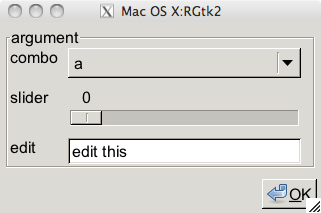
\includegraphics[width=0.45\textwidth]{ex-33-macosx-rgtk2} &
    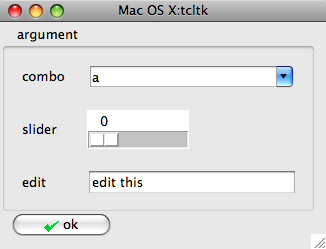
\includegraphics[width=0.45\textwidth]{fig-gWidgets-ex-33-tlctk}\\
    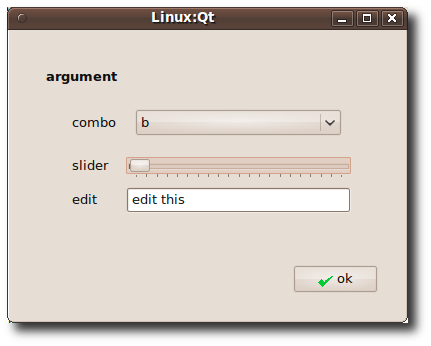
\includegraphics[width=0.45\textwidth]{ex-33-linux-qt} &
    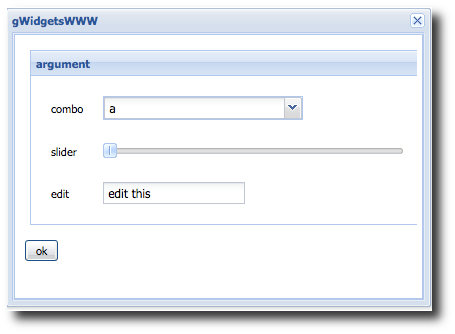
\includegraphics[width=0.45\textwidth]{ex-33-gWidgetsWWW}
  \end{tabular}
  \caption{The \pkg{gWidgets} package works with different operating
    systems and different GUI toolkits. This shows, the same code using the
    \pkg{RGtk2}, \pkg{tcltk}, \pkg{qtbase} packages for a toolkit. Additionally,
    the \pkg{gWidgetsWWW} package is used in the lower right figure.}
  \label{fig:gWidgets-three-oses}
\end{figure}

% %% Make figure -- work on layout here
% \XXX{Do mac, windows}
% \begin{figure}
%   \centering
%   \begin{tabular}{lccc}
%     & \pkg{RGtk2} & \pkg{tcltk} & \pkg{rJava} 
%     \\
%     L &
%     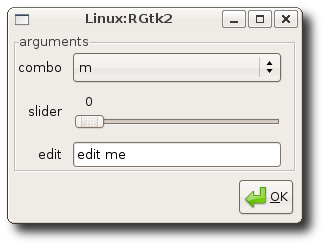
\includegraphics[width=0.3\textwidth]{ex-33-linux-rgtk2.png} &
%     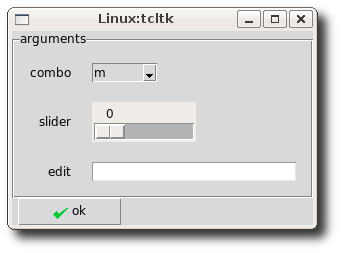
\includegraphics[width=0.3\textwidth]{ex-33-linux-tcltk} &
%     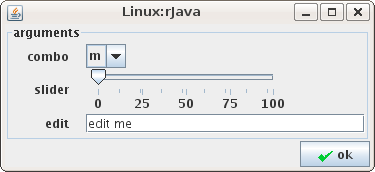
\includegraphics[width=0.3\textwidth]{ex-33-linux-rJava} 
%     \\
%     W &
%     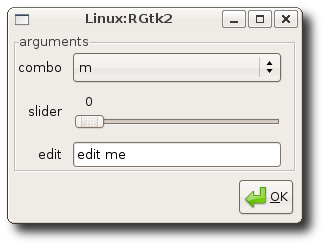
\includegraphics[width=0.3\textwidth]{ex-33-linux-rgtk2} &
%     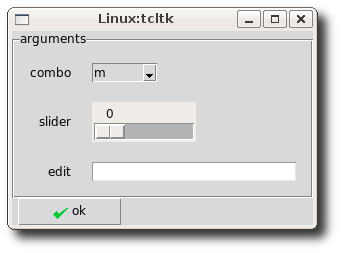
\includegraphics[width=0.3\textwidth]{ex-33-linux-tcltk} &
%     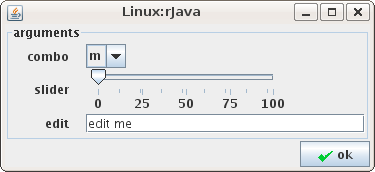
\includegraphics[width=0.3\textwidth]{ex-33-linux-rJava} 
%     \\
%     Mac &
%     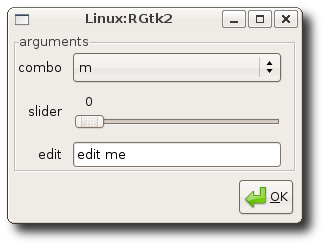
\includegraphics[width=0.3\textwidth]{ex-33-linux-rgtk2} &
%     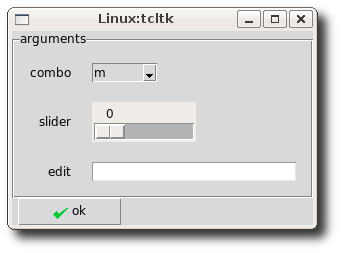
\includegraphics[width=0.3\textwidth]{ex-33-linux-tcltk} &
%     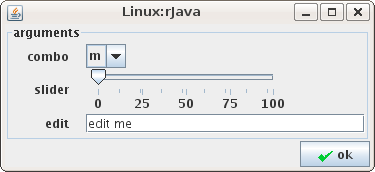
\includegraphics[width=0.3\textwidth]{ex-33-linux-rJava}
%   \end{tabular}
%   \caption{The \pkg{gWidgets} package works with different operating systems and different GUI toolkits. This shows the combination of \code{linux}, \code{Mac OS X (10.5)} and \code{Windows XP} and the packages \pkg{RGtk2}, \pkg{tcltk}, and \pkg{rJava}}
%   \label{fig:three-oses-three-toolkits}
% \end{figure}


% \begin{figure}
%   \centering
%   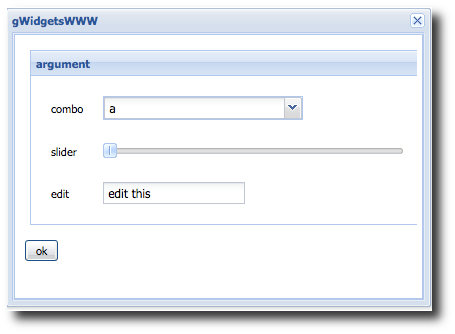
\includegraphics[width=.45\textwidth]{ex-33-gWidgetsWWW}
%   \caption{A GUI shown using \pkg{gWidgetsWWW}.}
%   \label{fig:gWidgetsWWW-same-gui}
% \end{figure}





\section{Constructors}
\label{sec:constructors}

We jump right in with an example~\footnote{Many thanks to Richie
  Cotton for suggesting this example and its follow up in
  Example~\ref{eg-gwidgets-file-system-II}.} leaving comments about
installation to the end of the chapter. The following shows some
sample \pkg{gWidgets} commands that set up a basic interface allowing
a user to search their hard drive for files matching a user-specified
pattern. The first line loads the package, the others will be
described later.

% <<>>=
% require(gWidgets)
% options(guiToolkit="RGtk2")

% w <- gwindow("Text input example", visible=FALSE)
% g <- ggroup(container=w)
% l <- glabel("Your name:", cont=g)
% e <- gedit("", cont=g)
% b <- gbutton("Click", cont=g, handler=function(h,...) {
%   msg <- sprintf("Hello %s", svalue(e))
%   cat(msg, "\n")
% })
% #
% visible(w) <- TRUE
% @ 

\begin{figure}
  \centering
  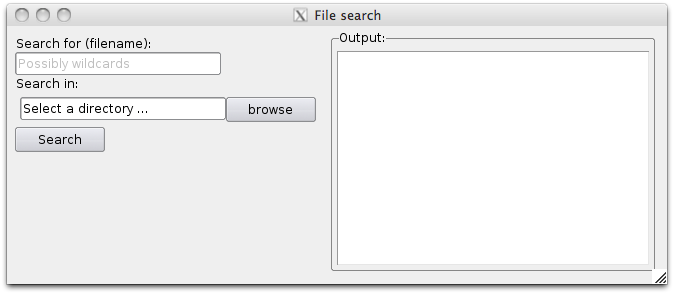
\includegraphics[width=.8\textwidth]{fig-file-search.png}
  \caption{A simple GUI for search for files matching a pattern. This
    GUI uses a paned group to separate the controls for searching from
    the results.}
  \label{fig:file-search}
\end{figure}

\begin{Schunk}
\begin{Sinput}
 require(gWidgets)
 options(guiToolkit="RGtk2")
 ## 
 w <- gwindow("File search", visible=FALSE)
 g <- gpanedgroup(cont=w)
 ## label and file selection widget
 f <- ggroup(cont=g, horizontal=FALSE)
 glabel("Search for (filename):", cont=f, anchor=c(-1,0))
 txtPattern <- gedit("", initial.msg="Possibly wildcards", cont=f)
 ##
 glabel("Search in:", cont=f, anchor=c(-1,0))
 startDir <- gfilebrowse(text="Select a directory ...",
                         quote=FALSE,
                         type="selectdir", cont=f)
 ## A button to initiate the search
 searchBtn <- gbutton("Search", cont=f)
 addSpring(f)
 ## Area for output
 f1 <- gframe("Output:", cont=g, horizontal=FALSE)
 searchResults <- gtext("", cont=f1, expand=TRUE)
 size(searchResults) <- c(350, 200)
 ## add interactivity
 addHandlerChanged(searchBtn, handler=function(h,...) {
   pattern <- glob2rx(svalue(txtPattern))
   fnames <- dir(svalue(startDir), pattern, recursive=TRUE)
   if(length(fnames))
     svalue(searchResults) <- fnames
   else
     galert("No matching files found", parent=w)
 })
 ## display GUI
 visible(w) <- TRUE
\end{Sinput}
\end{Schunk}

This example shows several different widgets being used to construct a
GUI, as seen in Figure~\ref{fig:file-search}. For example, on the
left is a text entry widget (\code{gedit}), a directory browsing
widget (\code{gfilebrowse}) and a button (\code{gbutton}). On the
right, is a multi-line text widget (\code{gtext}) in a framed
container (\code{gframe}).

The widgets are all produced by calling the appropriate constructor.
In the \pkg{gWidgets} API most of these constructors have the
following basic form:
\begin{Schunk}
\begin{Sinput}
 gname(arguments, handler = NULL, action = NULL, 
       container=NULL, ..., toolkit=guiToolkit())
\end{Sinput}
\end{Schunk}
where the \code{arguments} vary depending on the object being made. We
discuss now the common arguments.

\paragraph{container}
In the above, we see that the \code{gwindow} constructor, for a
top-level window, has two arguments passed in, an unnamed one for a
window title and a value for the \code{visible} property. Whereas the
\code{gpanedgroup} constructor takes all the default arguments except for
the parent container.

%% container
A top-level window does not have a parent container, but other GUI
components do. In \pkg{gWidgets}, for the sake of portability, the
parent container is passed to the widget constructor through the
\args{container} argument, as it done in all the other constructors.
This argument name can always be abbreviated \args{cont}. This nesting
defines the GUI layout, a topic taken up in
Chapter~\ref{sec:gWidgets-Containers}.

%% toolkit
\paragraph{toolkit}
The \args{toolkit} argument is usually not specified. It is there to
allow the user to mix toolkits within the same \R\/ session, but in
practice this can cause problems due to competing event loops. 
In our example we have 
\begin{Schunk}
\begin{Sinput}
 options(guiToolkit="RGtk2")
\end{Sinput}
\end{Schunk}
%
to explicitly set the toolkit. The default for the \args{toolkit}
argument though is to call to \function{guiToolkit}. This function
will check if a toolkit has been specified, or only one is
available. If neither case is so, then a menu will be provided for the
user to choose one.

\paragraph{handler, action}
The \args{handler} and \code{action} arguments are used to pass in
event handlers. We discuss those in Section~\ref{sec:callbacks}.


%% return value
\paragraph{Side effects}
The constructors produce one of three general types of widgets:
\begin{description}
\item[Containers] such as the top level window \code{w}, the paned
  group \code{g} or the frame \code{f1}
 (Table~\ref{tab:gWidgets-container-constructors});
%
\item[Components] such as the unnamed labels, the edit area
  \code{txtPattern},, or the button \code{searchBtn}
  (Tables~\ref{tab:gWidgets-control-widgets}
  and~\ref{tab:gWidgets-compound-widgets});
%
\item[Dialogs] such as \code{galert} and \code{gfilebrowse} (Table~\ref{tab:gWidgets-basic-dialogs}).
\end{description}



%% container argument
% ML: this has already been well explained in preceeding chapters
% A GUI consists of a hierarchical nesting of containers. Each container
% may contain contain controls or additional containers. In a GUI,
% except for top-level windows (including dialogs), every component and
% container is the child of some parent container. 

% ML: This sounds to me that it is a detail of specific toolkit implementations
% The package does not implement layout managers. Rather, in
% the construction of a widget in \pkg{gWidgets}, the
% \meth{add} method for the parent container is called with the new
% object as an argument and the values passed through the \args{...}
% argument as arguments.  


% We remark that not all the toolkits (e.g., \pkg{RGtk2}, \pkg{qtbase})
% require one to combine the construction of an object with the
% specification of the parent container. We don't illustrate this, as
% the resulting code is not cross-toolkit.

% % toolkit argument
% The \code{toolkit} can be specified at time of construction allowing
% toolkits, in theory, to be mixed. Otherwise, the \code{guiToolkit}
% function returns the currently selected toolkit, or queries for one if
% none is selected.  Constructors dispatch on the \code{toolkit} value
% to call the appropriate constructor in the toolkit implementation. The
% return value from the toolkit's constructor is kept in the
% \code{widget} component.

\section{Methods}


In addition to creating a GUI object, most \pkg{gWidgets}'
constructors also return a useful \R\/ object. This is an S4 object of
a certain class containing two components: \code{toolkit} and
\code{widget}. (Modal dialogs do not return an object, as the dialog
will be destroyed before the constructor returns. Instead, their
constructors return values reflecting the user response to the
dialog.)


GUI objects have a state determined by one or more of their
properties. In \pkg{gWidgets} many properties are set at the time of
construction. However, there are also several new generic methods defined
for \pkg{gWidgets} objects to adjust these properties.~\footnote{ We
  are a bit imprecise about the term ``method'' here. The
  \pkg{gWidgets} methods call further methods in the underlying
  toolkit interface which we think of a single method call. The actual
  S4 object has a slot for the toolkit and the widget created by the
  toolkit interface to dispatch on.  }

%% s3 generics
Depending on the class of the object, the \pkg{gWidgets} package
provides methods for the familiar S3 generics \generic{[},
\generic{[$<$-}, \generic{dim}, \generic{length}, \generic{names},
\generic{names$<$-}, \generic{dimnames}, \generic{dimnames$<$-} and
\generic{update}.


%% svalue
In our example, we see two cases of the use of generic methods defined
by \pkg{gWidgets}. The call
\begin{Schunk}
\begin{Sinput}
 svalue(txtPattern)
\end{Sinput}
\end{Schunk}
%
demonstrates the new generic \index{svalue}{\meth{svalue}} that is used to get
the main property of the widget. For the object \code{txtPattern}, the
main property is the text, for the button and label widgets this
property is the label. The \index{svalue\ASSIGN}\meth{svalue\ASSIGN} assignment method is
used to set this property programatically. We see the call
\begin{Schunk}
\begin{Sinput}
 svalue(searchResults) <- fnames
\end{Sinput}
\end{Schunk}
to update the text for the multi-line text widget \code{searchResults}.

%% selection widgets
For the selection widgets (which we don't have in our example), there
is a natural mapping between vectors or data frames, and the data to
be selected. In this case, the user may want the value selected or the
index of the selected value. The \args{index=TRUE} argument of
\meth{svalue} may be specified to refer to values by their index. 

%% [, [<- method
For these selection widgets the familiar \meth{[} and \meth{[\ASSIGN}
methods refer to the underlying data to be selected from.



The call
\begin{Schunk}
\begin{Sinput}
 visible(w) <- TRUE
\end{Sinput}
\end{Schunk}
%
sets the visibility property of the top-level window. In our example,
the \code{gwindow} constructor is passed \code{visible=FALSE} to
suppress an initial drawing of the window, making this call to
\meth{visible\ASSIGN} necessary to show the GUI. The
\code{visible\ASSIGN} generic has different interpretations for the
various widgets.

Some other methods to adjust the widget's underlying properties are
\meth{font\ASSIGN}, to adjust the font of an object; \meth{size} and
\meth{size\ASSIGN} to query and set the size of a widget; and
\meth{enabled\ASSIGN}, to adjust if a widget is sensitive to user
input.

%% tag and tag<- need not be advertised here. They are too hacky.
% %% tag; tag<-
% The methods \meth{tag} and
% \meth{tag\ASSIGN} are similar to the base \function{attr}
% function. However, the attributes persist across copies of the
% object. These are implemented to bypass the pass-by-copy issues that
% can make GUI programming awkward at times.

%% insufficiency of API
The \pkg{gWidgets} API provides just a handful of generic functions
for manipulating an object's properties compared to the number of
methods typically provided by a GUI toolkit for a similar
object. Although this simplicity makes \pkg{gWidgets} easier to work
with, one may wish to get access to the underlying toolkit object to
take advantage of a richer API. In most cases, the
\generic{getToolkitWidget} will provide that object. We don't
illustrate this here, as we try to stay toolkit agnostic in our
examples.


%% table of new methods
\begin{table}
\centering
\label{tab:gWidgets-methods}
\caption{Generic functions provided or used in the \pkg{gWidgets} API.}
\begin{tabular}{@{}lp{0.6\textwidth}@{}}
\toprule

Method&Description\\
\midrule
\meth{svalue, svalue\ASSIGN}&Get or set widget's main property\\\meth{size\ASSIGN}&Set preferred size request of widget in pixels\\\meth{show}&Show widget if not visible\\\meth{dispose}&Destroy widget or its parent\\\meth{enabled, enabled\ASSIGN}&Adjust sensitivity to user input\\\meth{visible, visible\ASSIGN}&Show or hide object or part of object.\\\meth{focus\ASSIGN}&Set focus to widget\\\meth{insert}&Insert text into a multi-line text widget\\\meth{font\ASSIGN}&Set a widget's font\\\meth{update}&Update widget value\\\meth{isExtant}&Does \R\/ object refer to GUI object that still exists\\&\\\meth{[, [\ASSIGN}&Refers to values in data store\\\meth{length}&\meth{length} of data store\\\meth{dim}&\meth{dim} of data store\\\meth{names}&\meth{names} of data store \\\meth{dimnames}&\meth{dimnames} of data store\\&\\\meth{getToolkitWidget}&Return underlying toolkit widget for low-level use
\\ \bottomrule
\end{tabular}
\end{table}% \begin{table}
%   \centering
%   \begin{tabular}{l@{\quad}p{.75\textwidth}}
% %    \toprule
%     \meth{svalue, svalue\ASSIGN} & Get or set value for widget\\
%     \meth{[, [\ASSIGN} & If widget has a data store, refers to these values \\
%     \meth{length} & \meth{length} of data store\\
%     \meth{dim} & \meth{dim} of data store\\
%     \meth{names} & \meth{names} of data store \\
%     \meth{dimnames} & \meth{dimnames} of data store\\
%     \meth{update} & update widget values\\
%     \meth{size\ASSIGN}& set size of widget in pixels\\
%     \meth{show}& show widget if not visible\\
%     \meth{dispose} & destroy widget or its parent\\
%     \meth{isExtant} & Does \R\/ object refer to GUI object that still exists\\
%     \meth{enabled, enabled\ASSIGN} & An enabled widget can receive input from the user\\
%     \meth{visible, visible\ASSIGN} & Is widget visible.\\
%     \meth{focus\ASSIGN} & Sets focus to widget\\
%     \meth{defaultWidget, defaultWidget\ASSIGN} & Makes widget have initial
%     focus in a dialog\\
%     \meth{insert} & Used to insert text into a multi-line text widget\\
%     \meth{font\ASSIGN} & Set the font for a widget\\
%     \meth{tag, tag\ASSIGN} & Sets an attribute for a widget that persists
%     through copies\\
%     \meth{id, id\ASSIGN} & A unique ID for a widget\\
%     \meth{getToolkitWidget} & Returns underlying toolkit widget for
%     low-level use\\
%     \bottomrule
%   \end{tabular}
%   \caption{Table of generic functions with methods specified by the \pkg{gWidgets} API.}
%   \label{tab:gWidgets-methods}
% \end{table}

\section{Event Handlers}
\label{sec:callbacks}

%% callbacks 

% For all the toolkits, when the user initiates some event with the
% mouse or keyboard, the underlying toolkit will emit some signal. The
% toolkits allow functions, referred to as callbacks, to be called when
% these signals are emitted, allowing the GUI to be made interactive.


In our example, the search button is created with:
\begin{Schunk}
\begin{Sinput}
 searchBtn <- gbutton("Search", cont=f)
\end{Sinput}
\end{Schunk}
%
However, without doing more work, this button will not initiate an
action. For that we need to add an event handler, or callback, to be
called when an event occurs. For our example, our event is a button
click and the action we want consists of several steps: turning our
pattern into a regular expression; searching for the specified
pattern; and presenting the results.  In our example, this is done
through:
\begin{Schunk}
\begin{Sinput}
 addHandlerChanged(searchBtn, handler=function(h,...) {
   pattern <- glob2rx(svalue(txtPattern))
   fnames <- dir(svalue(startDir), pattern, recursive=TRUE)
   if(length(fnames))
     svalue(searchResults) <- fnames
   else
     galert("No matching files found", parent=w)
 })
\end{Sinput}
\end{Schunk}
%
Callbacks in \pkg{gWidgets} have a common signature \code{(h,...)}
where \code{h} is a list with components \code{obj}, to pass in the
receiver of the event (the button in this case), and \code{action} to
pass along any value specified by the \args{action} argument (allowing
one to parameterize the callback).

For example, a typical idiom within a callback is
\begin{Schunk}
\begin{Sinput}
 prop <- svalue(h$obj)
\end{Sinput}
\end{Schunk}
%
which assigns the object's main property to \code{prop}.  We don't see
that above, as the values we desire belong to other widgets, which are
referred to through \R's usual scoping rules.  Some toolkits pass
additional arguments through the callback's \args{...}  argument, so
for portability this part of the signature is not optional. For some
handler calls, extra information is passed along through the list
\code{h}. For instance, in the drop target callback the component
\code{h\$dropdata} holds the drag-and-drop value.




Although it generally is best to keep separate the construction of the
widgets and the definition of the handlers, it is possible to pass in
a handler for the main event through the constructor's \args{handler}
argument. This argument, along with the \args{action} argument, will
be passed to the widget's \meth{addHandlerChanged} method. 


The package provides a number of generic methods
(Table~\ref{tab:gWidgets-callback-methods}) to add callbacks for
different events beyond \meth{addHandlerChanged}, which is used to
assign a callback for the typical event for the widget, such as the
clicking of a button. We refer to these methods as
``\meth{addHandlerXXX}'', where the \code{XXX} describes the
event. These are useful in the case where more than one event on that
widget is of interest. For example, for single-line text widgets, like
\code{txtPattern} in our example, the \meth{addHandlerChanged} method
sets a callback to respond when the user finishes editing, whereas a
handler set by \meth{addHandlerKeystroke} is called each time a key is
pressed.

As an example of combining the handler and constructor, we could have
specified the search button through:
\begin{Schunk}
\begin{Sinput}
 searchBtn <- gbutton("Search", cont=f,
              handler=function(h,...) {
                pattern <- glob2rx(svalue(h$action$txt))
                fnames <- dir(svalue(h$action$dir), 
                              pattern, recursive=TRUE)
                if(length(fnames))
                  svalue(h$action$results) <- fnames
                else
                  galert("No matching files found", parent=w)
              },
              action=list(txt=txtPattern, dir=startDir,
                results=searchResults)
              )
\end{Sinput}
\end{Schunk}
%
By passing in the other widgets through the \code{action} argument one
can avoid worrying about any potential issues with scope.

The \meth{addHandlerXXX} methods return an ID.  This ID can be used
with the method \meth{removeHandler} to remove the callback, or with
the methods \meth{blockHandler} and \meth{unblockHandler} to
temporarily block a handler from being called.

If these few methods are insufficient and toolkit-portability is not
of interest, then the \meth{addHandler} generic can be used to specify
a toolkit-specific signal and a callback.


\begin{table}
\centering
\label{tab:gWidgets-callback-methods}
\caption{Generic functions to add callbacks in \pkg{gWidgets} API.}
\begin{tabular}{@{}lp{0.6\textwidth}@{}}
\toprule

Method&Description\\
\midrule
\meth{addHandlerChanged}&Primary handler call for when a widget's value is "changed." The interpretation of "change" depends on the widget.\\\meth{addHandlerClicked}&Set handler for when widget is clicked with (left) mouse button. May return position of click through components \code{x} and \code{y} of the \code{h}-list. \\\meth{addHandlerDoubleclick}&Set handler for when widget is double clicked\\\meth{addHandlerRightclick}&Set handler for when widget is right clicked\\\meth{addHandlerKeystroke}&Set handler for when key is pressed. The \code{key} component is set to this value, if possible.\\\meth{addHandlerFocus}&Set handler for when widget gets focus\\\meth{addHandlerBlur}&Set handler for when widget loses focus\\\meth{addHandlerExpose}&Set handler for when widget is first drawn\\\meth{addHandlerUnrealize}&Set handler for when widget is undrawn on screen\\\meth{addHandlerDestroy}&Set handler for when widget is destroyed\\\meth{addHandlerMouseMotion}&Set handler for when widget has mouse go over it\\\meth{addDropSource}&Specify a widget as a drop source\\\meth{addDropMotion}&Set handler to be called when drag event mouses over the widget\\\meth{addDropTarget}&Set handler to be called on a drop event. Adds the component \code{dropdata}.\\\meth{addHandler}&(Not cross-toolkit) Allows one to specify an underlying signal from the graphical toolkit and handler\\&\\\meth{removeHandler}&Remove a handler from a widget\\\meth{blockHandler}&Temporarily block a handler from being called\\\meth{unblockHandler}&Restore handler that has been blocked\\\meth{addHandlerIdle}&Call a handler during idle time\\&\\\meth{addPopupmenu}&Bind popup menu to widget\\\meth{add3rdMousePopupmenu}&Bind popup menu to right mouse click
\\ \bottomrule
\end{tabular}
\end{table}


\section{Dialogs}
\label{sec:gWidgets-modal-dialogs}

The \pkg{gWidgets} package provides a few constructors to quickly make
some basic dialogs for showing messages or gathering
information. Mostly these are modal dialogs that take control of the
event loop, not allowing any other part of the GUI to be active for
programmatic interaction. As such, in \pkg{gWidgets}, constructors of
modal dialogs do not return an object to manipulate through its
methods, but rather return the user response to the dialog. For example, the
\code{gfile} dialog, described later, is a modal dialog that pops up a
means to select a file returning the selected file path or
\code{NA}. It is used along the lines of:
\begin{Schunk}
\begin{Sinput}
 if(!is.na(f <- gfile())) source(f)
\end{Sinput}
\end{Schunk}



\begin{table}
\centering
\label{tab:gWidgets-basic-dialogs}
\caption{Table of constructors for basic dialogs in \pkg{gWidgets}}
\begin{tabular}{@{}lp{0.7\textwidth}@{}}
\toprule

Constructor&Description\\
\midrule
\constructor{gmessage}&Dialog to show a message\\\constructor{galert}&Unobtrusive (non-modal) dialog to show a message\\\constructor{gconfirm}&Confirmation dialog\\\constructor{ginput}&Dialog allowing user input\\\constructor{gbasicdialog}&Flexible modal dialog\\\constructor{gfile}&File and directory selection dialog
\\ \bottomrule
\end{tabular}
\end{table}% \begin{table}
%   \centering
%  \begin{tabular}{l@{\quad}p{.75\textwidth}}
% %   \toprule
%     \constructor{gfile} & File and directory selection dialog\\
%     \constructor{gmessage} & Dialog to show a message\\
%     \constructor{galert} & Unobtrusive (non-modal) dialog to show a message\\
%     \constructor{gconfirm} & Confirmation dialog\\
%     \constructor{ginput} & Dialog allowing user input\\
%     \constructor{gbasicdialog} & Flexible modal dialog \\
%     \bottomrule
%   \end{tabular}
%   \caption{Table of basic dialogs in \pkg{gWidgets}}
%   \label{tab:gWidgets-modal-dialogs}
% \end{table}


In the example, we use two non-modal dialogs \code{gfilebrowse} to
select a directory and \code{galert} to display a transient message if
no files are found through our search.  Here we describe the dialogs
that can be used to display a message or gather a simple amount of
text. The \constructor{gfile} dialog is described in
Section~\ref{sec:gWidgets-selecting-from-file} and the
\constructor{gbasicdialog}, which is implemented like a container, is
described in Section~\ref{sec:modal-window}.


The information dialogs are simple one-liners. For example, this
command will cause a confirmation dialog to popup allowing the user to
select a value which will be returned as \code{TRUE} or \code{FALSE}:
\begin{Schunk}
\begin{Sinput}
 gconfirm("Yes or no? Click one.")
\end{Sinput}
\end{Schunk}


The information dialogs have arguments \argument{message}{gmessage}
for a message; \argument{title}{gmessage} for the window title; and
\argument{icon}{gmessage} to specify an icon, whose value is one of
\qcode{info}, \qcode{warning}, \qcode{error}, or
\qcode{question}. Buttons will appear at the bottom of the dialog, and
are determined by choice of the constructor. The
\argument{parent}{gmessage} argument is used to position the dialog
near the \pkg{gWidgets} instance specified. Otherwise, placement will
be controlled by the window manager.

The dialogs, except for \code{galert}, have the standard
\code{handler} and \code{action} arguments, for calling a handler, but
typically it is easier to use the return value when programming.

\paragraph{A message dialog}
The simplest dialog is produced by \code{gmessage}, which
displays a message. The user has a cancel button to dismiss the dialog.


For example,
\begin{Schunk}
\begin{Sinput}
 gmessage("Message goes here", title="example dialog")
\end{Sinput}
\end{Schunk}


\paragraph{An alert dialog}
The \code{galert} dialog is similar to \code{gmessage} only it is
meant to be less obtrusive, so it is non-modal. It does not take the
focus and vanishes after a time delay.

\paragraph{A confirmation dialog}
The constructor \constructor{gconfirm} produces a dialog that allows
the user to confirm the message. This dialog returns \code{TRUE} or
\code{FALSE} depending on the user's selection.


Here we use the question icon for a confirmation dialog, as the message is a question.
\begin{Schunk}
\begin{Sinput}
 ret <- gconfirm("Really delete file?", icon="question")
\end{Sinput}
\end{Schunk}


\paragraph{An input dialog}
The \constructor{ginput} constructor produces a dialog which allows
the user to input a single line of text. If the user confirms the
dialog, the value of the string is returned, otherwise if the user
cancels the dialog through the button a value of \code{NA} is returned.


This illustrates how to use the return value.
\begin{Schunk}
\begin{Sinput}
 ret <- ginput("Enter your name", icon="info")
 if(!is.na(ret)) 
   message("Hello", ret,"\n")
\end{Sinput}
\end{Schunk}


% \begin{example}{Modal dialogs}{ex-gWidgets-modal-dialogs}
%   \SweaveInput{ex-gWidgets-modal-dialogs}
% \end{example}





\section{Installation}
\label{sec:installation}



The \pkg{gWidgets} package interfaces with an underlying \R\/ package
through an intermediate package. For example,
Figure~\ref{fig:gWidgets-yuml} shows the sequence of calls to produce
a button. First the \pkg{gWidgets} package dispatches to a toolkit
package (\pkg{gWidgetsRGtk2}), which in turn calls functions in the
underlying \R\/ package (\pkg{RGtk2}) which in turn calls into the
graphical toolkit to produce an object. This is then packaged into an
S4 object to manipulate.~\footnote{The S4 object consists of a
  \pkg{gWidgets} object and a toolkit reference. The \pkg{gWidgets}
  package simply provides generic functions that dispatch down to a
  toolkit counterpart using this S4 object. The actual class
  structure, methods and their inheritance is within the toolkit
  package. (This allows one to follow the class structure of the
  underlying graphical library.) As such, \pkg{gWidgets} simply
  provides an interface (in the sense of constructors and methods to
  implement) for the toolkit packages to implement. Any discussion to
  classes, methods and inheritance for \pkg{gWidgets} here then is for
  simplicity of exposition.}

As such, to use \pkg{gWidgets} with the \GTK\/ toolkit one must have
installed on their computer the GTK\/ libraries, the \pkg{RGtk2}
package and the \pkg{gWidgetsRGtk2} package and the \pkg{gWidgets}
package.


\begin{figure}
  \centering
  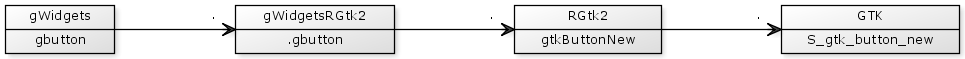
\includegraphics[width=.95\textwidth]{fig-gWidgets-yuml}
  \caption{The construction of a button widget in \pkg{gWidgets}
    requires several steps}
  \label{fig:gWidgets-yuml}
\end{figure}
%% From
%%http://yuml.me/diagram/class/[gWidgets%7Cgbutton]-.%3E[gWidgetsRGtk2%7C.gbutton],%20[gWidgetsRGtk2%7C.gbutton]-.%3E[RGtk2%7CgtkButtonNew],%20[RGtk2%7CgtkButtonNew]-.%3E[GTK%7CS_gtk_button_new]


The difficulty for the end user is the installation of the graphic
toolkit, as all other packages are installed through CRAN, or are
recommended packages with an \R\/ installation
(\pkg{tcltk}). Table~\ref{tab:gWidgets-installation} roughly describes
the installation process for different operating systems and
toolkits. For Windows users, some details are linked to in the \R{}
for Windows FAQ.

%% JV Perhaps this belongs somewhere else in the text...
\begin{table}
\centering
\label{tab:gWidgets-installation}
\caption{Installation notes for GUI toolkits.}
\begin{tabular}{@{}lp{0.3\textwidth}p{0.3\textwidth}p{0.3\textwidth}@{}}
\toprule

&Gtk+&Qt&Tk\\
\midrule
Windows&Download exe file&Install libraries, binary&In binary install of R\\Linux&Standard&Standard&Standard\\OS X&Download binary .pkg&Install from vendor&In binary install of R
\\ \bottomrule
\end{tabular}
\end{table}
Not all features of the \pkg{gWidgets} API are implemented for a
toolkit. In particular, the easiest to install toolkit package
(\pkg{gWidgetstcltk}) might have the fewest features, as the \code{Tk}
libraries are not as featureful.  The help pages in the \pkg{gWidgets}
package describe the API, with the help pages in the toolkit packages
indicating differences or omissions from the API
(e.g. \code{?gWidgetsRGtk2-package}). For the most part, omissions are
gracefully handled by simply providing less functionality.

% %% starting package
% The \pkg{gWidgets} package is loaded as other \R\/ packages:
% <<>>=
% require(gWidgets)
% @ 

% A toolkit package is loaded when the first command is issued. If a
% user does not have a toolkit installed, a message instructs the user
% to install one.

% %% Choice of toolkit
% If a user has exactly one toolkit package installed, then that will be
% used. But it is possible for more than one to be installed, in which
% case the user is prompted to choose one through an interactive menu. This
% choice can be avoided by setting the option \args{guiToolkit} to the
% \code{XXX} in a \pkg{gWidgestXXX} package name, e.g.,
% <<>>=
% options("guiToolkit"="RGtk2")
% @ 

% Although in theory the different toolkits can be used
% together, in practice the different event loops created by each often
% lead to issues that can lockup the \R\/ process.



\chapter{\pkg{gWidgets}: Container Widgets}
\label{sec:gWidgets-Containers}
%% Basic Containers

%% ML: Might be clearer if the examples came almost at the beginning
%% of each section and followed by the details. For me, it's much
%% easier to see something and then have it explained, instead of
%% reading the details, constructing the example in my imagination,
%% and then seeing it.

% \begin{table}
%   \centering
%   \begin{tabular}{l@{\quad}p{.75\textwidth}}
% %    \toprule
%     \constructor{gwindow} & Creates a top-level window\\
%     \constructor{ggroup} & Creates a box-like container\\
%     \constructor{gframe} & Creates a container with a text label \\
%     \constructor{gexpandgroup} & Creates a container with a label and
%     expand/collapse trigger\\ 
%     \constructor{gpanedgroup} & Creates a container for two child widgets
%     with a handle to assign allocation of space\\
%     \constructor{glayout} & A grid container\\
%     \constructor{gnotebook} & A tabbed notebook container for holding a
%     collection of child widgets\\
%     \bottomrule
%   \end{tabular}
%   \caption{Table of container constructors in \pkg{gWidgets}}
%   \label{tab:gWidgets-container-constructors}
% \end{table}


After identifying the underlying data to manipulate and how to
represent it, GUI construction involves three basic steps:
\begin{itemize}
\item creation and configuration of the main components;
\item the layout of these components; and
\item connecting the components through callbacks to make a GUI interactive.
\end{itemize}

This chapter discusses the layout process within
\pkg{gWidgets}. Layout in \pkg{gWidgets} is done by placing child
components within parent containers which in turn may be nested in
other containers.~\footnote{This is more like \GTK, and not \Qt, where
  layout managers control where the components are displayed.} In our
file search example from the previous chapter, we nested a framed box
container inside a paned container inside a top level window.  

The \pkg{gWidgets} package provides a just few types of containers:
top-level windows (\code{gwindow}), box containers (\code{ggroup},
\code{gframe}, \code{gexpandgroup}), a grid container
(\code{glayout}), a paned container (\code{gpanedgroup}) and a
notebook container
(\code{gnotebook}). Figure~\ref{fig:gWidgets-sample-layout} shows most
all of these employed to produce a GUI to select and then show the
contents of a file.


%% add
In some toolkits, notably \pkg{tcltk}, the widget constructors require
the specification of a parent container for the widget. To accomodate
that, the \pkg{gWidgets} constructors -- except for top-level windows
and dialogs -- have the argument \args{container} to specify the
immediate parent container.  Within the constructor is the call
\code{add(container, child, ...)} where the constructor creates the
child and \code{...}  values are passed from the constructor down to
the \meth{add} method.  That is, the widget construction and layout
are coupled together. Although, this isn't necessary when utilizing
\pkg{RGtk2} or \pkg{qtbase} -- and the two aspects can be separated --
for the sake of cross-toolkit portability we don't illustrate this
style here.



\begin{figure}
  \centering
  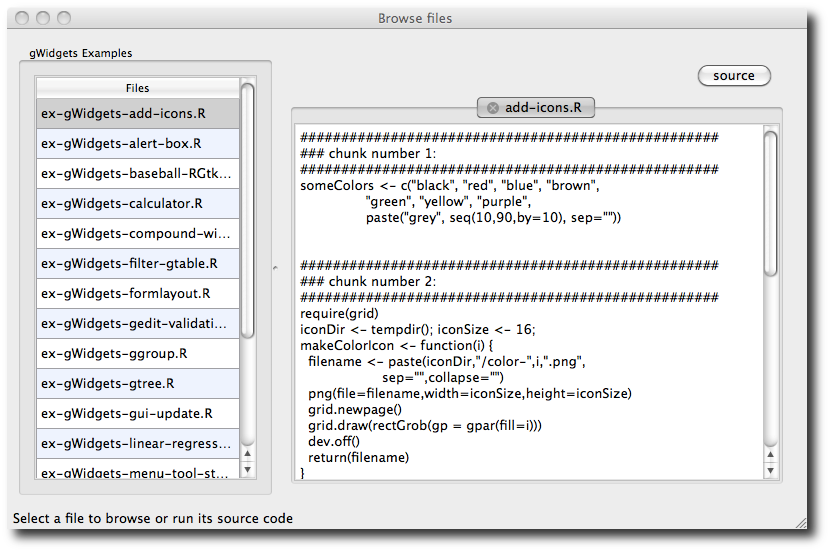
\includegraphics[width=.8\textwidth]{fig-gWidgets-example-browser}
  \includegraphics[width=.8\textwidth]{fig-example-browser-schematic.png}
  \caption{The example browser for gWidgets showing different layout
    components. The lower image shows the different containers used.}
  \label{fig:gWidgets-sample-layout}
\end{figure}



\section{Top-level windows}
\label{sec:gWidgets-top-level-windows}

The \constructor{gwindow} constructor creates top-level windows. The
main window property is the title which is typically displayed in the
window's title bar. This can be set during construction via the
\argument{title}{gwindow} argument or accessed later through the object's
\meth{svalue\ASSIGN} method. A basic window then is constructed as follows:

\begin{Schunk}
\begin{Sinput}
 w <- gwindow("Our title", visible=TRUE)
\end{Sinput}
\end{Schunk}
%

We can then use this as a parent container for a constructor. For example;
\begin{Schunk}
\begin{Sinput}
 l <- glabel("A child label", container=w)
\end{Sinput}
\end{Schunk}
%
However, top-level windows only allow one child component. Typically,
this child is a container, such as a box container, allowing for
multiple children.


%% visible
The optional \argument{visible}{gwindow} argument, used above with its
default value \code{TRUE}~\footnote{If the option
  \code{gWidgets:gwindow-default-visible-is-false} is non NULL, then
  the default will be \code{FALSE}.}, controls whether the window is
initially drawn. If not drawn, the \method{visible\ASSIGN}{gwindow}
method, taking a logical value, can be used to draw the window later.
Often it is good practice to suppress the initial drawing, especially
for displaying GUIs with several controls, as the incremental drawing
of subsequent child components can make the GUI seem sluggish. As
well, this allows the underlying toolkit to compute the necessary size
before it is displayed.~\footnote{For \pkg{gWidgetstcltk} the \meth{update}
method will initiate this recomputation. This may be necessary to get the
window to size properly.}

For example, a typical usage follows this pattern:
\begin{Schunk}
\begin{Sinput}
 w <- gwindow("Title", visible=FALSE)
 ## perform layout here ...
 visible(w) <- TRUE
\end{Sinput}
\end{Schunk}

%% Size and placement
\paragraph{Size and placement}
In GUI programming, a window geometry is a specification of position
and size, often abbreviated $w \times h + x + y$. The width and height
can be specified at construction through the \argument{width}{gwindow}
and \argument{height}{gwindow} arguments. This initial size is the
default size, but may be adjusted later through the
\method{size}{gwindow} method or through the window manager. 

%% parent, location
The initial placement of a window, $x+y$, will be decided by the
window manager, unless the \argument{parent}{gwindow} argument is
specified. If this is done with a vector of $x$ and $y$ pixel values,
the upper left corner will be placed at this point. The \args{parent}
argument can also be another \code{gwindow} instance. In this case,
the new window will be positioned over the specified window and be
transient for the window. That is, it will be disposed when the parent
window is. This is useful, say, when a main window opens a dialog
window to gather values.

For example this call makes a child window of \code{w} with a square
size of 200 pixels.
\begin{Schunk}
\begin{Sinput}
 childw <- gwindow("A child window", parent=w, 
                   width=200, height=200)
\end{Sinput}
\end{Schunk}


%% dispose/addHandlerUnrealize
\paragraph{Handlers}
Windows objects can be closed programmatically through their
\method{dispose}{gwindow} method. Windows may also be closed through
the window manager, by clicking a close icon in the title bar. The
default event is the close event. For example, the following will add
in a call to \code{galert} when an error occurs until the window is closed:

%% Thanks to Richie Cotton for this example
\begin{Schunk}
\begin{Sinput}
 oldOptions <- options(error = function() {
   if(msg <- geterrmessage() != "")
     galert(msg, parent=win)
   invisible(msg)
 })
 #
 win <- gwindow( "Popup errors", visible=FALSE,
                handler = function(h, ...) {
                  ## restore old options when gui is closed
                  options(oldOptions)       
                })
\end{Sinput}
\end{Schunk}

To illustrate, we add a button to initiate an error:
\begin{Schunk}
\begin{Sinput}
 btn <- gbutton("Click for error",  cont = win,
                handler = function(h, ...) {
                  stop("This is an error")
                })
\end{Sinput}
\end{Schunk}
%
Clicking the button will signal an error and the error handler will
display an alert popup. (This last part fails under \pkg{tcltk} due to
that packages handling of errors in callbacks.)


The \argument{handler}{gwindow} argument is called just before the
window is destroyed, but cannot prevent that from happening.  The
\method{addHandlerUnrealize}{gwindow} method can be used to call a
handler between the initial click of the close icon and the subsequent
destroy event of the window. This handler must return a logical value:
if \code{TRUE} the window will not be destroyed, if \code{FALSE} the
window will be. For example:

\begin{Schunk}
\begin{Sinput}
 w <- gwindow("Close through the window manager")
 id <- addHandlerUnrealize(w, handler=function(h,...) {
   !gconfirm("Really close", parent=h$obj)
 })
\end{Sinput}
\end{Schunk}

In most GUIs,  the use of menubars, toolbars and
status bars is often reserved for the main window, while dialogs are
not decorated so.  In \pkg{gWidgets} it is suggested, although not
strictly enforced unless done so by the underlying toolkit, that these be
added only to a top-level window.  We discuss these widgets later in
Section~\ref{sec:gWidgets-acti-menus-toolb}. 

\begin{table}
\centering
\label{tab:gWidgets-container-constructors}
\caption{Constructors for container objects}
\begin{tabular}{@{}lp{0.6\textwidth}@{}}
\toprule

Constructor&Description\\
\midrule
\constructor{gwindow}&Creates a top-level window\\\constructor{ggroup}&Creates a box-like container\\\constructor{gframe}&Creates a box container with a text label\\\constructor{gexpandgroup}&Creates a box container with a label and trigger to expand/collapse\\\constructor{glayout}&A grid container\\\constructor{gpanedgroup}&Creates a container for two child widgets with a handle to assign allocation of space.\\\constructor{gnotebook}&A tabbed notebook container for holding a collection of child widgets
\\ \bottomrule
\end{tabular}
\end{table}





\subsection{A modal window}
\label{sec:modal-window}


The \constructor{gbasicdialog} constructor allows one to place an
arbitrary widget within a modal window. It also adds \kbd{OK} and
\kbd{Cancel} buttons, unless the argument
\argument{do.buttons}{gbasicdialog} is specified as \code{FALSE}. The argument \argument{title}{gbasicdialog} is
used to specify the window title.



As with the \function{gconfirm} dialog, this widget returns
\code{TRUE} or \code{FALSE} depending on the user's selection. To do
something more complicated than \code{gconfirm}, a handler should be
specified at construction which is called just before the dialog is
disposed.


This dialog is used in a slightly different manner, requiring the use
of a call to \meth{visible} (not \meth{visible\ASSIGN}).
There are three basic steps: an initial call to
\function{gbasicdialog} to return a container to be used as the parent
container for a child component; a construction of the dialog; then a
call to the \code{visible} method on the dialog with \code{set=TRUE}
value. The dialog is closed through clicking one of its buttons,
through a window manager event, or programmatically through its
\method{dispose}{gbasicdialog} method.

In Example~\ref{eg:gWidgets-collapse-factor} we define a GUI to assist
with the task of collapsing factor levels. This wrapper function is used:

\begin{Schunk}
\begin{Sinput}
 collapseFactor <- function(f, parent=NULL) {
   out <- character()
   w <- gbasicdialog("Collapse factor levels", parent=parent,
                     handler=function(h,...) {
                       new_f <- relf$get_value()
                       out <<- factor(new_f)
                     })
   g <- ggroup(cont=w)
   relf <- CollapseFactor$new(f, cont=g)
   visible(w, set=TRUE)
   out
 }
\end{Sinput}
\end{Schunk}

By wrapping the \code{gbasicdialog} call within a function, we can
return the factor, not just a logical, so the above can be used as
\begin{Schunk}
\begin{Sinput}
 mtcars$am <- collapseFactor(mtcars$am)
\end{Sinput}
\end{Schunk}



\section{Box containers}
\label{sec:gWidgets-box-containers}

The container produced by \constructor{gwindow} is intended to contain
just a single child widget, not several. This section demonstrates
variations on box containers that can be used to hold multiple child
components. Through nesting, fairly complicated layouts can be
produced.



\begin{table}
\centering
\label{tab:gWidgets-container-methods}
\caption{Container methods}
\begin{tabular}{@{}lp{0.6\textwidth}@{}}
\toprule

Method<&Description\\
\midrule
\meth{add}&Adds a child object to a parent container. Called when a parent container is specified to the \args{container} argument of the widget constructor, in which case, the \args{...} arguments are passed to this method.\\\meth{delete}&Remove a child object from a parent container\\\meth{dispose}&Destroy container and children\\\meth{enabled\ASSIGN}&Set sensitivity of child components\\\meth{visible\ASSIGN}&Hide or show child components
\\ \bottomrule
\end{tabular}
\end{table}


\subsection{The \code{ggroup} container}
\label{sec:gWidgets-ggroup-container}
  
The basic box container is produced by \constructor{ggroup}. Its main
argument is \argument{horizontal}{ggroup} to specify whether the child
widgets are packed in horizontally from left to right (the default) or
vertically from top to bottom. 

For example, to pack a \code{cancel} and \code{ok} button into a box container we might have:
\begin{Schunk}
\begin{Sinput}
 w <- gwindow("Some buttons", visible=FALSE)
 g <- ggroup(horizontal=TRUE, cont=w)
 cancel <- gbutton("cancel", cont=g)
 ok <- gbutton("ok", cont=g)
 visible(w) <- TRUE
\end{Sinput}
\end{Schunk}

\paragraph{The add method}
When packing in child widgets, the \method{add}{ggroup} method is
used. In our example above, this is called by the
\code{gbutton} constructor when the \args{container} argument is
specified.~\footnote{In this text, the \meth{add} method is typically called
from the constructor, but there are two cases where one calls it
directly. The first is if one wishes to integrate a widget from the
underlying graphical toolkit into a \pkg{gWidgets} GUI. An example
where the \pkg{tkrplot} package is embedded in a GUI is given in 
Section~\ref{sec:gWidgets-graphics-device}. The second case, is when a
widget is removed from a GUI through \meth{delete}. In most cases it
may be added back in with \meth{add}.}Unlike with the underlying graphical toolkits, there is no
means to specify other styles of packing such as from the ends, or in
the middle by some index.

The \meth{add} method for box containers has a few arguments to
customize where the child widgets are placed and how they respond when
their parent window is resized. These are passed through the
\args{...}  argument of the
constructor. Figure~\ref{fig:gWidgets-ggroup-expand-fill-anchor} shows
some differences in how these argument are
implemented.~\footnote{These arguments are not implemented
  consistently across toolkits, as the underlying toolkit may prevent
  it. For example, for \pkg{RGtk2} the child widgets always fill in
  the direction opposite of how they are added (horizontal widgets
  always fill top to bottom), where as for \pkg{tcltk} widgets will
  fill only if the \code{expand} argument is \code{TRUE}.}

\begin{description}
\item[expand, fill] The underlying layout algorithms have a means to
  allocate space to child widgets when the parent container
  expands. Those widgets which have \code{expand=TRUE}
  specified should get the excess space shared amongst
  them. (This isn't the case in \code{gWidgetsQt}, where a \code{fill}
    value needs to be specified as well.)
 

\item[fill, anchor] When a child widget is placed into its allocated
  space, the space is generally large enough to accommodate the
  child. If there is additional space, it can be desirable that that
  the widget grow to fill the available space.  The \code{fill}
  argument, taking a value of \code{x}, \code{y} or \code{both} (also
  \code{TRUE}) indicates how the widget should fill any additional
  allocation (only when \code{expand=TRUE}).~\footnote{For \GTK,
    filling always occurs orthogonally to the direction of
    packing. This is why the top and bottom buttons (when
    \code{expand=FALSE}) in
    Figure~\ref{fig:gWidgets-ggroup-expand-fill-anchor} for
    \pkg{gWidgetsRGtk2} stretch across the container. To avoid this
    filling, pack the button in a horizontal \code{ggroup} container.}
 
  If a widget does not expand or if it does but does not fill in both
  directions, it can be anchored into its available space in more than
  one position. The \args{anchor} argument can be specified to suggest
  where to anchor the child. It takes a numeric vector representing
  Cartesian coordinates (length two),
  with either value being \code{-1}, \code{0}, or \code{1}. For
  example, a value of \code{c(1,1)} would specify the northwest corner.
\end{description}

\begin{figure}
  \centering
  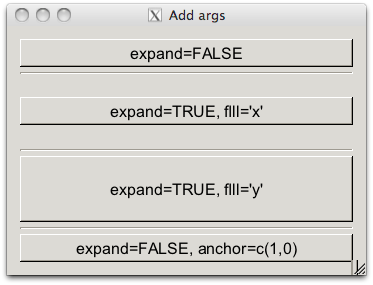
\includegraphics[width=.3\textwidth]{fig-gWidgets-expand-RGtk2.png}
  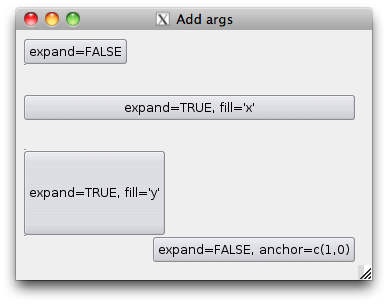
\includegraphics[width=.3\textwidth]{fig-gWidgets-expand-tcltk.png}
  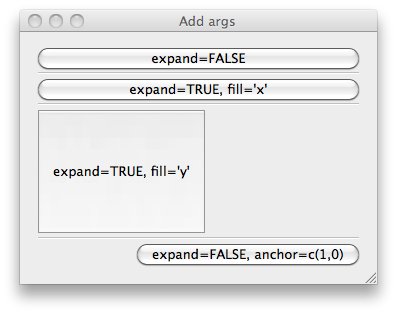
\includegraphics[width=.3\textwidth]{fig-gWidgets-expand-Qt.png}
  % 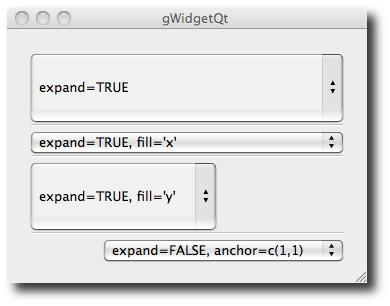
\includegraphics[width=.5\textwidth]{fig-gWidgets-ggroup-expand-fill-anchor}
  % \caption{Different combinations of \code{expand}, \code{fill} and
  %   \code{anchor} for combo boxes in \pkg{gWidgetsQt}. The \code{fill}
  %   and \code{anchor} arguments
  %   may be overridden by the underlying toolkit for some widgets.}
  \caption{
    The \args{expand}, \args{fill}, and \args{anchor} arguments are
    implemented slightly differently in the different
    packages. (\pkg{gWidgetsRGtk2} on left, \pkg{gWidgetstctlk} in
    middle and \pkg{gWidgetsQt} on right.). For \GTK\/ child
    components packed in a box container always fill in the direction
    opposite the packing, in this case the ``x'' direction. As such,
    the \code{anchor} directive has no effect. For
    \pkg{tcltk} a widget only fills if \code{expand=TRUE} is given.
    For \pkg{gWidgetsQt} expansion and fill are linked together.
  }
  \label{fig:gWidgets-ggroup-expand-fill-anchor}
\end{figure}


\paragraph{delete}
The \method{delete}{ggroup} method can be used to remove a child
component from a container. In some toolkits, this child may be added
back at a later time (with \method{add}{ggroup}), but this isn't part
of the API. In the case where you wish to hide a child temporarily,
its \meth{visible\ASSIGN} method may usually be used, although some
widgets give this method a different meaning.~\footnote{In
  \pkg{gWidgetstcltk} the use of \meth{visible\ASSIGN} to hide a
  component is not supported.}





\paragraph{Spacing}
For spacing between the child components, the constructor's argument
\argument{spacing}{ggroup} may be used to specify, in pixels, the
amount of space between the child widgets. For \code{ggroup}
instances, this can later be set through the \method{svalue}{ggroup}
method. The method \method{addSpace}{ggroup} can add a non-uniform
amount of space between two widgets packed next to each other, whereas
the method \method{addSpring}{ggroup} will place an invisible spring
between two widgets, forcing them apart.  Both are useful for laying
out buttons. We used a spring before the ``source'' button for the GUI
in Figure~\ref{fig:gWidgets-sample-layout} to push it to the right.


For example, we might modify our button layout example to include a
``help'' button on the far left and the others on the right with a
fixed amount of space between them as follows (Figure~\ref{fig:gWidgets-button-layout}):
\begin{Schunk}
\begin{Sinput}
 w <- gwindow("Some buttons", visible=FALSE)
 g <- ggroup(horizontal=TRUE, spacing=6, cont=w)
 help <- gbutton("help", cont=g)
 addSpring(g)
 cancel <- gbutton("cancel", cont=g)
 addSpace(g, 12)                         # 6 + 12 + 6 pixels
 ok <- gbutton("ok", cont=g)
 visible(w) <- TRUE
\end{Sinput}
\end{Schunk}


\begin{figure}
  \centering
  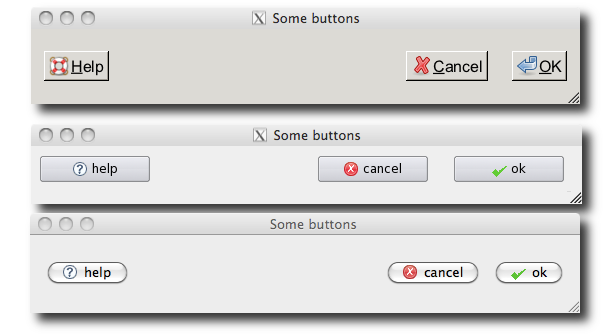
\includegraphics[width=.7\textwidth]{fig-gWidgets-buttons}
  \caption{Button layout for \pkg{RGtk2} (top), \pkg{tcltk} (middle)
    and \pkg{qtbase} (bottom). Although the same code is used for each, the different styling yields varying sizes. }
  \label{fig:gWidgets-button-layout}
\end{figure}

% To illustrate how the right panel of
% Figure~\ref{fig:gWidgets-sample-layout} was done, we used nested
% layouts as follows:

% <<echo=FALSE>>=
% w <- gwindow("Nested layout example")
% @ 

% <<nestedLayout, results=hide>>=
% g <- ggroup(horizontal=FALSE, cont=w)
% bg <- ggroup(cont=g)                    # nested group
% addSpring(bg)
% b <- gbutton("Source", cont=bg)
% nb <- gnotebook(cont=g, expand=TRUE)    # fill space
% @ 


\paragraph{Sizing}
The overall size of a \code{ggroup} container is typically decided by
how it is added to its parent. However, a requested size can be assigned
through the \method{size\ASSIGN}{ggroup} method. 


For some toolkits the argument \argument{use.scrollwindow}{ggroup},
when specified as \code{TRUE}, will add scrollbars to the box
container so that a fixed size can be maintained. Setting a requested
size in this case is a good idea. (Although it is generally
considered a poor idea to use scrollbars when there is a chance the
key controls for a dialog will be hidden, this can be useful for
displaying lists of data.)


% \begin{example}{The \args{use.scrollwindow} argument}{ex-gWidgets-ggroup-use.scrollwindow}
%   \SweaveInput{ex-gWidgets-ggroup-scrollwindow}
% \end{example}

% The next example shows an alternative to the expand group widget.

% \begin{example}{The \meth{delete} method of \code{ggroup}}{ex-gWidgets-ggroup-delete}
%   \SweaveInput{ex-gWidgets-alert-box}
% \end{example}


\subsection{The \code{gframe} and \code{gexpandgroup} containers}
\label{sec:gWidgets-decorated-cont}

We discuss briefly two widgets that essentially subclass the
\code{ggroup} class. Much of the previous discussion applies.

Framed containers are used to set off its child elements using a
border and label. The \constructor{gframe} constructor produces
them. In Figure~\ref{fig:gWidgets-sample-layout} the table to select
the file is nested in a frame to give the user some indication
as to what to do.

For \constructor{gframe} the first argument, \argument{text}{gframe}, is
used to specify the label. This can later be adjusted through the
\method{names\ASSIGN}{gframe} method. The argument
\argument{pos}{gframe} can be specified to adjust the label's
positioning with $0$ being the left and $1$ the right.



The basic framed container is used along these lines:
\begin{Schunk}
\begin{Sinput}
 w <- gwindow("gframe example")
 f <- gframe("gWidgets Examples:", cont=w)
 files <- list.files(system.file("Examples","ch-gWidgets", 
                                 package="ProgGUIInR"))
 vars <- gtable(files, cont=f, expand=TRUE)
\end{Sinput}
\end{Schunk}


Expandable containers are useful when their child items need not be
visible all the time. The typical design involves a trigger indicator
with accompanying label indicating to the user that a click can
disclose or hide some additional information.~\footnote{How each
  toolkit resizes when the widget collapse varies, so using this
  container can cause layout issues if cross-toolkit portability is an
  issue.}  This class essentially subclasses \code{gframe} where the
\method{visible\ASSIGN}{gexpandgroup} method is overridden to initiate
the hiding or showing of its child area, not the entire container.

In addition, a handler can be added that is called whenever the widget
toggles its state.

Here we show how one might leave optional the display of a statistical
summary of a model.
\begin{Schunk}
\begin{Sinput}
 res <- lm(mpg ~ wt, mtcars)
 out <- capture.output(summary(res))
 w <- gwindow("gexpandgroup example", visible=FALSE)
 xgrp <- gexpandgroup("Summary", cont=w)
 l <- glabel(out, cont=xgrp)
 visible(xgrp) <- TRUE                   # display summary
 visible(w) <- TRUE
\end{Sinput}
\end{Schunk}


\paragraph{Separators}
Although not a container, the \constructor{gseparator} widget can be
used to place a horizontal or vertical line (with the
\code{horizontal=FALSE} argument) in a layout to separate off parts of
the GUI. 




% \begin{example}{The \constructor{gframe} and \constructor{gexpandgroup} containers}{gWidgets-gframe-gexpandgroup-ex}
% \SweaveInput{ex-gWidgets-gframe-gexpandgroup.Rnw}
% \end{example}



\section{Grid layout: the \code{glayout} container}
\label{sec:gWidgets-glayout-container}

The layout of dialogs and forms is usually seen with some form of
alignment between the widgets. The \constructor{glayout} constructor
provides a grid container to do so, using matrix notation to specify
location of the children.  

To see its use, we can layout a simple form for collecting information
as follows:

\begin{Schunk}
\begin{Sinput}
 w <- gwindow("glayout example", visible=FALSE)
 lyt <- glayout(cont=w, spacing=5)
 right <- c(1,0); left <- c(-1,0)
 lyt[1,1, anchor=right] <- "name"
 lyt[1,2, anchor=left ] <- gedit("", cont=lyt)
 #
 lyt[2,1, anchor=right] <- "rank"
 lyt[2,2, anchor=left ] <- gedit("", cont=lyt)
 #
 lyt[3,1, anchor=right] <- "serial number"
 lyt[3,2, anchor=left ] <- gedit("", cont=lyt)
 visible(w) <- TRUE
\end{Sinput}
\end{Schunk}
%

When adding a child, in addition to being on the left hand side of the
\code{[\ASSIGN} call, the \code{glayout} container should be specified
as the widget's parent \code{container}.~\footnote{This is necessary
  only for the toolkits where a container must be specified, where the
  right hand side is used to pass along the parent information and the
  left hand side is used for the layout.} For convenience, if the
right hand side is a string, a label will be generated.  To align a
widget within a cell, the \argument{anchor}{add} argument of the
\code{[\ASSIGN}{glayout} method is used. The example above illustrates
how this can be used to achieve a center balance.

The constructor has a few arguments to configure the appearance of the
container. The spacing between each cell may be specified through the
\argument{spacing}{glayout} argument, the default is 10 pixels. A
value of 5 is used above to tighten up the display.
To impose a uniform cell size, the \argument{homogeneous}{glayout}
argument can be specified with a value of \code{TRUE}. The default is
\code{FALSE}. 

As seen, children may be added to the grid at a specific row and
column. To specify this, \R's matrix notation, \code{[\ASSIGN}, is
used with the indices indicating the row and column.  A child may span
more than one row or column. The corresponding index should be a
contiguous vector of indices indicating so.  

The \code{[} method may be used to return the children. This methods
returns a single item, a list of items or a matrix of items. To return
the main properties of the widgets in the above example can be done
through:
\begin{Schunk}
\begin{Sinput}
 sapply(lyt[,2], svalue)
\end{Sinput}
\begin{Soutput}
[1] "" "" ""
\end{Soutput}
\end{Schunk}



% \begin{example}{Layout with \constructor{glayout}}{ex-gWidgets-glayout}
%   This example shows how a simple form can be given an center-balanced
%   layout using a grid container. 

% \end{example}


\section{Paned containers: the \code{gpanedgroup} container}
\label{sec:gWidgets-gpanedgroup-container}

The \constructor{gpanedgroup} constructor produces a container which
has two children separated by a visual gutter that can be
adjusted by the user with their mouse to allocate the space between them.
Figure~\ref{fig:gWidgets-sample-layout} uses such a
container to separate the file selection controls from the file
display ones.  For this container, the children are aligned
side-by-side (by default) or top to bottom if the
\argument{horizontal}{gpanedgroup} argument is given as
\code{FALSE}. 


To add children, the container should be used as the parent container
for two constructors. These can be other container constructors which
is the typical usage for more complicated layouts.
(For toolkits which support the separation of widget
construction and layout, the \constructor{gpanedgroup} constructor can
have two children specified to the arguments
\argument{widget1}{gpanedgroup} and \argument{widget2}{gpanedgroup}.)

The main property of this container is the sash position, a value in
$[0,1]$. This may be configured programmatically through the
\method{svalue\ASSIGN}{gpanedgroup} method. A value from 0 to 1
specifies the proportion of space allocated to the leftmost (topmost)
child. This specification only works after the containing window is
drawn, as the percentage is based on the size of the window.


A simplified version of the layout in
Figure~\ref{fig:gWidgets-sample-layout} would be
\begin{Schunk}
\begin{Sinput}
 d <- system.file("Examples", "ch-gWidgets", 
                  package="ProgGUIinR")
 files <- list.files(d)
 #
 w <- gwindow("gpanedgroup example", visible=FALSE)
 pg <- gpanedgroup(cont = w)
 tbl <- gtable(files, cont=pg)           # left side
 t <- gtext("", cont=pg, expand=TRUE)    # right side
 visible(w) <- TRUE
 svalue(pg) <- 0.33                      # after drawing
\end{Sinput}
\end{Schunk}


% \begin{example}{Paned groups}{ex-gWidgets-panedgroups}
%   This example shows how one could use this container.
% <<keep.source=TRUE>>=
% w <- gwindow("gpanedgroup example", visible=FALSE)
% pg <- gpanedgroup(cont=w)
% g <- ggroup(cont=pg)                  # left child
% l <- glabel("left child", cont=g)
% b <- gbutton("right child", cont=pg)
% visible(w) <- TRUE
% @ 
% To adjust the sash position, one can do:
% <<>>=
% svalue(pg) <- 0.75
% @ 
% \end{example}


  
\section{Tabbed notebooks: the \code{gnotebook} container}
\label{sec:gWidgets-gnotebook}

The \constructor{gnotebook} constructor produces a tabbed notebook
container. The GUI in Figure~\ref{fig:gWidgets-sample-layout} uses a
notebook to hold different text widgets, one for each file being displayed.

The constructor has a few arguments, not all supported by each
toolkit. The argument \argument{tab.pos}{gnotebook} is used to specify
the location of the tabs using a value of 1 through 4 with 1 being
the bottom, 2 the left side, 3 the top and 4 the right side, with the
default being 3 (similar numbering as used in \function{par}). The
\argument{closebuttons}{gnotebook} argument takes a logical indicating
whether the tabs should have close buttons on them. In this case, the
argument \argument{dontCloseThese}{gnotebook} can be used to specify
which tabs, by index, should not be closable.



\paragraph{Methods}
Pages are added through the \method{add}{gnotebook} method for the
notebook container. The extra  \argument{label}{add} argument is used
to specify the tab label. (As \meth{add} is called implicitly when a a
widget is constructed, this argument is usually specified to the
constructor.)



The \method{svalue}{gnotebook} method returns the index of the
currently raised tab, whereas \method{svalue\ASSIGN}{gnotebook} can be
used to switch the page to the specified tab. The currently shown tab
can be removed using the \method{dispose}{gnotebook} method. To remove
a different tab, use this method in combination with
\meth{svalue\ASSIGN}. (When removing many tabs, you will want to start
from the end as otherwise the tab positions change during removal.)

From some viewpoint, the notebook widget is viewed as a vector with a
names attribute (the labels) and components being the child
components. As such, the \meth{[} method returns the the child
components (by index), the \method{names}{gnotebook} method refers to
the tab names, and the \method{length}{gnotebook} method returns the
number of pages held by the notebook.



\begin{example}{Tabbed notebook example}{ex-gWidgets-gnotebook}
 In the GUI of Figure~\ref{fig:gWidgets-sample-layout} a notebook is
 used to hold differing pages. The following is the basic setup used.
\begin{Schunk}
\begin{Sinput}
 w <- gwindow("gnotebook example")
 nb <- gnotebook(cont=w)
\end{Sinput}
\end{Schunk}

New pages are added as follows:
\begin{Schunk}
\begin{Sinput}
 addAPage <- function(fname) {
   f <- system.file(fname, package="ProgGUIinR")
   gtext(readLines(f), cont = nb, label=fname)
 }
 addAPage("DESCRIPTION")
\end{Sinput}
\end{Schunk}

For pages holding more than one widget, a container is used:
\begin{Schunk}
\begin{Sinput}
 hg <- glayout(cont=nb, horizontal=FALSE, label="Help")
 hg[1,1] <- gimage("help", dir="stock", cont=hg)
 hg[1,2] <- glabel(paste("To add a page:",
              "Click on a file in the left pane, and its contents",
              "are displayed in a notebook page.", sep="\n"), 
              cont=hg)
\end{Sinput}
\end{Schunk}


To manipulate the displayed pages, say to set the page to the last one
we have:
\begin{Schunk}
\begin{Sinput}
 svalue(nb) <- length(nb)
\end{Sinput}
\end{Schunk}
%
To remove the current page
\begin{Schunk}
\begin{Sinput}
 dispose(nb)
\end{Sinput}
\end{Schunk}
%
\end{example}






\chapter{\pkg{gWidgets}: Control Widgets}
\label{cha:control-widgets}
%% organize by function

\XXX{Where to integrate methods such as enabled?}
\XXX{stock icons}
\XXX{addHandler text -- done here with first, but could be elsewhere}
\XXX{drag and drop example}
  

  
This Chapter discusses the basic GUI controls provided by
\pkg{gWidgets}. In the following one, we discuss some \R-specific widgets.

\begin{table}
\centering
\label{tab:gWidgets-control-widgets}
\caption{Table of constructors for control widgets in \pkg{gWidgets}. Most, but not all, are implemented for each toolkit.}
\begin{tabular}{@{}lp{0.7\textwidth}@{}}
\toprule

Constructor&Description\\
\midrule
\constructor{glabel}&A text label\\\constructor{gbutton}&A button to initiate an action \\\constructor{gcheckbox}&A checkbox\\\constructor{gcheckboxgroup}&A group of checkboxes\\\constructor{gradio}&A radio button group\\\constructor{gcombobox}&A drop-down list of values, possibly editable\\\constructor{gtable}&A table (vector or data frame) of values for selection\\\constructor{gslider}&A slider to select from a sequence value\\\constructor{gspinbutton}&A spinbutton to select from a sequence of values\\\constructor{gedit}&Single line of editable text\\\constructor{gtext}&Multi-line text edit area\\\constructor{ghtml}&Display text marked up with HTML\\\constructor{gdf}&Data frame viewer and editor\\\constructor{gtree}&A display for hierarchical data\\\constructor{gimage}&A display for icons and images\\\constructor{ggraphics}&A widget containing a graphics device\\\constructor{gsvg}&A widget to display SVG files\\\constructor{gfilebrowse}&A widget to select a file or directory\\\constructor{gcalendar}&A widget to select a date\\\constructor{gaction}&A reusable definition of an action\\\constructor{gmenubar}&Add a menubar on a top-level window \\\constructor{gtoolbar}&Add a toolbar to a top-level window\\\constructor{gstatusbar}&Add a status bar to a top-level window\\\constructor{gtooltip}&Add a tooltip to widget\\\constructor{gseparator}&A widget to display a horizontal or vertical line
\\ \bottomrule
\end{tabular}
\end{table}%% place these as appropriate
% \begin{table}
%   \centering
%   \begin{tabular}{l@{\quad}p{.75\textwidth}}
% %    \toprule
%     \constructor{glabel} & A text label\\
%     \constructor{gbutton} & A button to initiate an action \\
%     \constructor{gcheckbox} & A checkbox widget\\
%     \constructor{gradio} & Constructs a radio button group\\
%     \constructor{gcheckboxgroup} & Constructs a group of checkboxes\\
%     \constructor{gcombobox} & Constructs drop down list of values\\
%     \constructor{gtable} & Shows a table (vector or data frame) of
%     values for selection\\ 
%     \constructor{gslider} & A slider to select a value\\
%     \constructor{gspinbutton} & A spinbutton to select from a set of values\\
%     \constructor{gedit} & One line of editable text\\
%     \constructor{gtext} & multi-line text edit\\
%     \constructor{ghtml} & Display text marked up with HTML\\
%     \constructor{gdf} & Data frame viewer and editor\\
%     \constructor{gtree} & Displays hierarchical data\\
%     \constructor{gimage} & Displays icons and images\\
%     \constructor{ggraphics} & A widget containing a graphics device\\
%     \constructor{gfilebrowser} & A widget to select a file or directory\\
%     \constructor{gcalendar} & A widget to select a date\\
%     \constructor{gaction} & a reusable definition of an action\\
%     \constructor{gmenubar} & Puts a menubar on a top-level window\\    
%     \constructor{gtoolbar} & Adds a toolbar to a top-level window\\
%     \constructor{gstatusbar} & Adds a status bar to a top-level window\\
%     \constructor{gseparator} & A widget to display a horizontal or vertical line\\
%     \bottomrule
%   \end{tabular}
%   \caption{Table of basic control constructors in \pkg{gWidgets}}
%   \label{tab:gWidgets-control-widgets}  
% \end{table}


\subsection{Buttons}
\label{sec:gWidgets-buttons}

The button widget allows a user to initiate an action through clicking
on it. Buttons have labels, conventionally verbs indicating action,
and often icons. The \constructor{gbutton} constructor has an argument
\argument{text}{gbutton} to specify the text.  For text that matches
the stock icons of \pkg{gWidgets}
(Section~\ref{sec:gWidgets-displ-icons-imag}) an icon will
appear. (The \code{ok} button below, but not the \code{parButton} one.)

In common with the other controls, the argument
\argument{handler}{gbutton} is used to specify a callback and the
\argument{action}{gbutton} argument will be passed along to this
callback (unless it is a \code{gaction} object, whose case is
described in Section~\ref{sec:gWidgets-acti-menus-toolb}).  The
default handler is the click handler which can be specified at
construction, or afterward through
\method{addHandlerClicked}{gbutton}. The underlying toolkit's method
of invoking a callback through keyboard navigation is used.

The following example shows how a button can be used to call a sub
dialog to collect optional information. We imagine this as part of a
dialog to generate a plot.

\begin{Schunk}
\begin{Sinput}
 w <- gwindow("Make a plot")
 g <- ggroup(horizontal=FALSE, cont=w)
 glabel("... Fill me in ...", cont=g)
 bg <- ggroup(cont=g)
 addSpring(bg)
 parButton <- gbutton("par (mfrow) ...", cont=bg)
\end{Sinput}
\end{Schunk}
Our callback opens a subwindow to collect a few values for the
\code{mfrow} option.
\begin{Schunk}
\begin{Sinput}
 addHandlerClicked(parButton, handler=function(h,...) {
   w1 <- gwindow("Set par values for mfrow", parent=w)
   lyt <- glayout(cont=w1)
   lyt[1,1, align=c(-1,0)] <- "mfrow: c(nr,nc)"
   lyt[2,1] <- (nr <- gedit(1, cont=lyt))
   lyt[2,2] <- (nc <- gedit(1, cont=lyt))
   lyt[3,2] <- gbutton("ok", cont=lyt, handler=
                 function(h,...) {
                   x <- as.numeric(c(svalue(nr), svalue(nc)))
                   par(mfrow=x)
                   dispose(w1)
                 })
 })
\end{Sinput}
\end{Schunk}



%% methods
The button's label is its main property and can be queried or set with
\method{svalue}{gbutton} or \method{svalue\ASSIGN}{gbutton}.  Most
GUIs will make a button insensitive to user input if the button's
action is not currently permissible. Toolkits draw such buttons in a
grayed-out state. As with other components, the \method{enabled\ASSIGN}{gWidgets} method can set
or disable whether a widget can accept input.

%% Default
% A new button may or may not have the focus when a GUI is
% constructed. If it does have the focus, then the \kbd{return} key will
% initiate the button click signal. To make a GUI start with its focus
% on a button, the \method{defaultWidget}{gWidgets} method is available. 


% A basic example of a button with a handler was given in Example~\ref{ex-gWidgets-hello-world-button}.

%% ML: I don't think it would hurt to see something like that
%% again. The reader will expect an example here.

% As an example of the limitations of \pkg{gWidgets} compared to the
% underlying toolkits, within \pkg{gWidgets} there are no methods to set
% an icon, or add an mnemonic to the button.


% \begin{example}{Hello world button}{ex-gWidgets-hello-world-button}
%   This example shows how a button is assigned a handler to respond to
%   click events.~\footnote{Each toolkit has its idiosyncrasies. If this
%     example is run using \pkg{RGtk2} the button will stretch to fill
%     the space. At times this is not desired. Placing the button within
%     a \code{ggroup} container can prevent this. Whereas, under
%     \code{tcltk} the parent window will shrink to fit the button. The
%     \meth{size} method can prevent this if it is not desired.} When
%   working with handlers, one can use an object name that will be found
%   through \R's scoping rules, or the components passed through the
%   \code{h} argument, as below.

% <<>>=
% w <- gwindow("Button example")
% b <- gbutton("Click me", cont=w)
% id <- addHandlerChanged(b, action=w, handler=function(h,...) {
%   btnText <- svalue(h$obj)                   # or svalue(b)
%   svalue(h$obj) <- paste("don't", btnText, "again") # set text
%   enabled(h$obj) <- FALSE
%   svalue(h$action) <- "Button example is finished" # set title
% })

% @ 

% \end{example}


\subsection{Labels}
\label{asec:gWidgets-labels}

The \constructor{glabel} constructor produces a basic label
widget. We've already seen its use in a number of examples. The main
property, the label's text, is specified through the
\argument{text}{glabel} argument. This is a character vector of length
1 or is coerced into one by collapsing the vector with newlines. The
\method{svalue}{glabel} method will return the label text as a single
string, whereas the \method{svalue\ASSIGN}{glabel} method is
available to set the text programmatically.

The \method{font\ASSIGN}{glabel} method
can also be used to set the text markup
(Table~\ref{tab:gWidgets-font-properties}).~\footnote{For some of the underlying toolkits, setting the argument
\argument{markup}{glabel} to \code{TRUE} allows a native markup language
to be used (\GTK\/ had PANGO, \Qt\/ has rich text).}
\\

To make a form's labels have some emphasis we could do:
\begin{Schunk}
\begin{Sinput}
 w <- gwindow("label example")
 f <- gframe("Summary statistics:", cont=w)
 lyt <- glayout(cont=f)
 lyt[1,1] <- glabel("xbar:", cont=lyt)
 lyt[1,2] <- gedit("", cont=lyt)
 lyt[2,1] <- glabel("s:", cont=lyt)
 lyt[2,2] <- gedit("", cont=lyt)
 sapply(1:2, function(i) {
   tmp <- lyt[i,1]
   font(tmp) <- c(weight="bold", color="blue")
 })
\end{Sinput}
\end{Schunk}


The widget constructor also has the argument
\argument{editable}{glabel}, which when specified as \code{TRUE} will
add a handler to the event so that the text can be edited when the
label is clicked.  Although this is popular in some familiar
interfaces, such as a spreadsheet tab, it has not proven to be
intuitive to most users, as labels are not generally expected to change.

\subsection{HTML text}
\label{sec:html-text}

Not all toolkits have the native ability, but for those that do (\Qt) the
\constructor{ghtml} constructor allows HTML-formatted text to be
displayed, in a manner similar to \constructor{glabel}. This widget is
intended simply for displaying HTML-formatted pages. There are no
methods to handle the clicking of links, etc.

\subsection{Status bars}
\label{sec:gWidgets-statusbars}

In \pkg{gWidgets}, status bars are simply labels placed at the bottom of a
top-level window to leave informative, but non-disruptive, messages
for the user.  The \constructor{gstatusbar} constructor provides this
widget.  The \args{container} argument should be a top-level window
instance.  The only property is the label's text. This may be
specified at construction with the argument
\argument{text}{gstatusbar}. Subsequent changes are made through the
\method{svalue\ASSIGN}{gstatusbar} method.




\subsection{Displaying icons and images stored in files}
\label{sec:gWidgets-displ-icons-imag}

The \pkg{gWidgets} package provides a few stock icons that can be
added to various GUI components. A list of the defined stock icons is
returned by the function \code{getStockIcons}.  The names attribute
defines the valid stock icon names. It was mentioned that if a
button's label text matches a stock icon name, that icon will appear
adjacent to the label.



%% gimage
Other graphic files and the stock icons can be displayed by the
\constructor{gimage} widget. \footnote{Not all file types may be
  displayed by each toolkit, in particular \pkg{gWidgetstcltk} can
  only display gif, ppm, and xbm files.} The file to display is
specified through the \argument{filename}{gimage} argument of the
constructor. This value is combined with that of the
\argument{dirname}{gimage} argument to specify the file path.  Stock
icons are specified by using their name for the \code{filename}
argument and the character string \code{"stock"} for the
\code{dirname} argument.~\footnote{For \pkg{gWidgetsRGtk2}, the size
  of a stock icon can be adjusted through the \argument{size}{gimage}
  argument, with a value from \qcode{menu}, \qcode{small\_toolbar},
  \qcode{large\_toolbar}, \qcode{button}, or \qcode{dialog}.}
%% methods

The \method{svalue\ASSIGN}{gimage} method is used to change the
displayed file. In this case, a full path name is specified, or the
stock icon name.

The default handler is a button click handler.
\\

To illustrate, a simple means to embed a graph within a GUI is as follows:
\begin{Schunk}
\begin{Sinput}
 f <- tempfile()
 png(f)                                  # not gWidgetstcltk!
 hist(rnorm(100))
 dev.off()
 #
 w <- gwindow("Example to show a graphic")
 gimage(basename(f), dirname(f), cont=w)
\end{Sinput}
\end{Schunk}
%

More stock icon names may be added through the function
\code{addStockIcons}. This function requires a vector of stock icon
names and a vector of corresponding file paths, and is illustrated
through the following example.


\begin{example}{Adding and using stock icons}{ex-gWidgets-stock-icons}
This example shows how to add to the available stock icons and use
\code{gimage} to display them. It creates a table
(Figure~\ref{fig:gWidgets-stock-icons}) to select a color from, as an
alternative to a more complicated color chooser dialog.~\footnote{If
  \pkg{gWidgetstcltk} is used the image files would need to be
  converted to \code{gif} format, as \code{png} format is not a
  natively supported image type.}

\begin{figure}
  \centering
  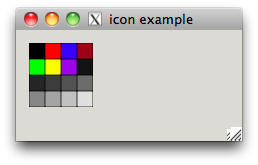
\includegraphics[width=.5\textwidth]{fig-gWidgets-icon-example.png}
  \caption{A table of stock icons created on the fly}
  \label{fig:gWidgets-stock-icons}
\end{figure}

We begin by defining 16 arbitrary colors.

\begin{Schunk}
\begin{Sinput}
 someColors <- c("black", "red", "blue", "brown",
                 "green", "yellow", "purple",
                 paste("grey", seq.int(10,90,by=10), sep=""))
\end{Sinput}
\end{Schunk}

This is the function that is used to create an icon file. We use some
low-level \pkg{grid} functions to draw the image to a png file.
\begin{Schunk}
\begin{Sinput}
 require(grid)
 iconDir <- tempdir(); iconSize <- 16;
 makeColorIcon <- function(i) {
   filename <- file.path(iconDir, 
                         sprintf("color-%s.png", i))
   png(file=filename, width=iconSize, height=iconSize)
   grid.newpage()
   grid.draw(rectGrob(gp=gpar(fill=i)))
   dev.off()
   return(filename)
 }
\end{Sinput}
\end{Schunk}

To add the icons, we need to define the stock names and the file paths
for \code{addStockIcons}.

\begin{Schunk}
\begin{Sinput}
 icons <- sapply(someColors, makeColorIcon)
 iconNames <- sprintf("color-%s", someColors)
 addStockIcons(iconNames, icons)
\end{Sinput}
\end{Schunk}

We use a table layout to show the 16 colors. As an illustration of
assigning a handler for a click event, we assign one that returns the
corresponding stock icon name.

\begin{Schunk}
\begin{Sinput}
 w <- gwindow("Icon example")
 f <- function(h,...) galert(h$action, parent=w)
 tbl <- glayout(cont=w, spacing=0)
 for(i in 1:4) {
   for(j in 1:4) {
     ind <- (i - 1) * 4 + j
     tbl[i,j] <- gimage(icons[ind], handler=f, 
                        action=iconNames[ind], cont=tbl)
   }
 }
\end{Sinput}
\end{Schunk}
\end{example}

\paragraph{SVG graphics}
Finally, we mention the \constructor{gsvg} constructor is similar to
\constructor{gimage}, but allows one to display SVG files, as produced
by the \function{svg} driver, say. It currently is not available for
\pkg{gWidgetsRGtk2} and \pkg{gWidgetstcltk}.


\section{Text editing controls}
\label{sec:gWidgets-text-edit-contr}
The \pkg{gWidgets} package, following the underlying toolkits, has two
main widgets for editing text: \constructor{gedit} for a single line
of editable text, and \constructor{gtext} for multi-line, editable
text. Each is simple to use, but provides much less flexibility than
is possible with the toolkit widgets.



\subsection{Single-line, editable text}
\label{sec:gWidgets-single-line-editable}


The \constructor{gedit} constructor produces a widget to display a
single line of editable text. The main property is the text which can
be set initially through the \argument{text}{gedit} argument.  If 
not specified, and the argument \argument{initial.msg}{gedit} is,
then this initial message is shown until the widget receives the focus
to guide the user.  If it is desirable to set the width of the widget,
the \argument{width}{gedit} argument allows the specification in terms
of number of characters allowed to display without horizontal
scrolling. The width of the widget may also be specified in pixel size
through the \method{size\ASSIGN}{guiWidget} method.
\\

A simple usage might be:
\begin{Schunk}
\begin{Sinput}
 w <- gwindow("Simple gedit example", visible=FALSE)
 g <- ggroup(cont=w)
 e <- gedit("", initial.msg="Enter your name...", cont=g)
 visible(w) <- TRUE
\end{Sinput}
\end{Schunk}



\paragraph{Methods}
The text is returned by the \method{svalue}{gedit} method and may be
set through the \method{svalue\ASSIGN}{gedit} method.  The
\meth{svalue} method will return a character vector by
default. However, it may be desirable to use this widget to collect
numeric values or perhaps some other type of variable. One could write
code to coerce the character to the desired type, but it is sometimes
convenient to have the return value be a certain non-character
type. In this case, the \argument{coerce.with}{gedit} argument can be
used to specify a function of a single argument to call before the
value is returned by \meth{svalue}.

The \method{visible}{gedit} method is overridden to mask out the
letters in the field, not hide the component. This allows one to use
the widget to collect passwords.

\paragraph{Auto completion}
The underlying toolkits offer some form of auto completion where the
entered text is matched against a list of values. These values
anticipate what a user wishes to type and a simple means to complete a
entry is offered. The \method{[\ASSIGN}{gedit} method allows these
values to be specified through a character vector, as in \code{obj[]
  \ASSIGN\/ values}.

For example, the following can be used to collect one of the 50 state
names in the U.S.:
\begin{Schunk}
\begin{Sinput}
 w <- gwindow("gedit example", visible=FALSE) 
 g <- ggroup(cont=w)
 glabel("State name:", cont=g)
 e <- gedit("", cont=g)
 e[] <- state.name
 visible(w) <- TRUE
\end{Sinput}
\end{Schunk}

\paragraph{Handlers}
The default handler for the \constructor{gedit} widget is called when
the text area is ``activated'' through the \kbd{return} key being
pressed. Use \meth{addHandlerBlur} to add a callback for the event of
losing focus. The \method{addHandlerKeystroke}{gedit} method can
assign a handler to be called when a key is released. For the toolkits
that support it, the specific key is given in the \code{key} component
of the list \code{h} (the first argument).~\footnote{There are
  differences in what keys are returned. Currently, only the letter
  keys are consistently given. In particular, no modifier keys or
  other keys are returned.}

\begin{example}{Validation}{ex-gWidgets-gedit-validation}
GUIs for \R\/ may differ a bit from many GUIs users typically
interact with, as \R\/ users expect to be able to use variables and
expressions where typically a GUI expects just characters or
numbers. As such, it is helpful to indicate to the user if their value
is a valid expression. This example shows how to implement a
validation framework on a single-line edit widget so that the user has
feedback when an expression will not evaluate properly.  When the
value is invalid we set the text color to red.


\begin{Schunk}
\begin{Sinput}
 w <- gwindow("Validation example")
 tbl <- glayout(cont=w)
 tbl[1,1] <- "R expression:"
 tbl[1,2] <- (e <- gedit("", cont = tbl))
\end{Sinput}
\end{Schunk}


We use the \pkg{evaluate} package to see if the expression is valid.
\begin{Schunk}
\begin{Sinput}
 require(evaluate)
 isValid <- function(e) {
   out <- try(evaluate:::evaluate(e), silent=TRUE)
   !(inherits(out, "try-error") ||  is(out[[2]], "error"))
 }
\end{Sinput}
\end{Schunk}
%

We validate our expression when the user commits the change, by
pressing the return key while the widget has focus. 

%% Just mentioned. If moved uncomment.
% Alternatively, we
% could have used
% \code{addHandlerKeystroke}, to validate after each key press, or
% \code{addHandlerBlur}, to validate when the widget loses focus.

\begin{Schunk}
\begin{Sinput}
 addHandlerChanged(e, handler = function(h,...) {
   curVal <- svalue(e)
   if(isValid(curVal)) {
     font(e) <- c(color="black")
   } else {
     font(e) <- c(color="red")
   }
 })
\end{Sinput}
\end{Schunk}

\end{example}

\subsection{Multi-line, editable text}
\label{sec:gWidgets-multi-line-editable}

The \constructor{gtext} constructor produces a multi-line text editing
widget with scrollbars to accommodate large amounts of text. The
\argument{text}{gtext} argument is for specifying the initial text. The
initial width and height can be set through similarly named
arguments. For widgets with scrollbars, specifying an initial size is
usually required as there otherwise is no indication as to how large
the widget should be.

The \method{svalue}{gtext} method retrieves the text stored in the
buffer. If the argument \code{drop=TRUE} is specified, then only the
currently selected text will be returned. Text in multiple lines is
returned as a single string with \qcode{\backslashn} separating the lines.

The contents of the text buffer can be replaced with the
\method{svalue\ASSIGN}{gtext} method. To clear the buffer, the
\method{dispose}{gtext} method may be used. The \method{insert}{gtext}
method adds text to a buffer. The signature is \code{insert(obj, text,
  where, font.attr)}
where \code{text} is a character vector. New text is added to the end
of the buffer, by default, but the \argument{where}{insert} argument
can specify \qcode{beginning} or \qcode{at.cursor}.





\begin{table}
\centering
\label{tab:gWidgets-font-properties}
\caption{Possible specifications for setting font properties. Font values of an object are changed with named vectors, as in \code{font(obj)\ASSIGN c(weight="bold", size=12, color="red")}}
\begin{tabular}{@{}lp{0.6\textwidth}@{}}
\toprule

Attribute&Possible value\\
\midrule
weight&light, normal, bold\\style&normal, oblique, italic\\family&normal, sans, serif, monospace\\size&a point size, such as 12\\color&a named color
\\ \bottomrule
\end{tabular}
\end{table}
\paragraph{Fonts}
Fonts can be specified for the entire buffer or the selection using
the specifications in Table~\ref{tab:gWidgets-font-properties}. To
specify fonts for the entire buffer use the
\argument{font.attr}{gtable} argument of the constructor. The
\method{font\ASSIGN}{gtext} method serves the same purpose, provided
there is no selection when called. If there is a selection, the font
change will only be applied to the selection. Finally, the
\argument{font.attr}{insert} argument for the \meth{insert} method
specifies the font attributes for the inserted text.
\\


As with \code{gedit}, the \method{addHandlerKeystroke}{gtext} method
sets a handler to be called for each keystroke. This is the default
handler.


\begin{example}{A calculator}{ex-gWidgets-calculator}
%% A calculator layout example

\begin{figure}
  \centering
  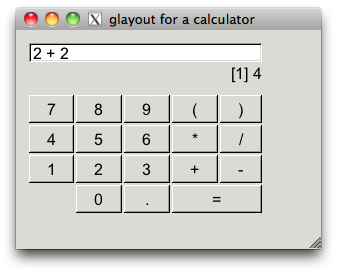
\includegraphics[width=.6\textwidth]{fig-gWidgets-calculuator.png}
  \caption{Dumbing down \R{} with \pkg{gWidgets} to make a calculator interface}
  \label{fig:gwidgets-calculator}
\end{figure}

This example shows how one might use the widgets just discussed to
make a GUI (Figure~\ref{fig:gwidgets-calculator}) that resembles a
calculator. Such a GUI may offer familiarity to new \R\/ users,
although certainly it is no replacement for a command line.

The \constructor{glayout} container is used to neatly arrange the
widgets. This example illustrates how a child widget can span a block
of multiple cells by using the appropriate indexing. Furthermore, the
\args{spacing} argument is used to tighten up the appearance. The
example also illustrates a useful strategy of storing the widgets
using a list for subsequent manipulations.

The following sets up the layout of the display and buttons.
\begin{Schunk}
\begin{Sinput}
 buttons <- rbind(c(7:9, "(", ")"),
                  c(4:6, "*", "/"),
                  c(1:3, "+", "-"))
 #
 w <- gwindow("glayout for a calculator", visible=FALSE)
 g <- ggroup(cont=w, expand=TRUE, horizontal=FALSE)
 tbl <- glayout(cont=g, spacing=2)
 tbl[1, 1:5, anchor=c(-1,0)] <-          # span 5 columns
   (eqnArea <- gedit("", cont=tbl))
 tbl[2, 1:5, anchor=c(1,0)] <- 
   (outputArea <- glabel("", cont=tbl))
 #
 bList <- list()
 for(i in 3:5) {
   for(j in 1:5) {
     val <- buttons[i-2, j]
     tbl[i,j] <- (bList[[val]] <- gbutton(val, cont=tbl))
   }
 }
 tbl[6,2] <- (bList[["0"]] <- gbutton("0", cont=tbl))
 tbl[6,3] <- (bList[["."]] <- gbutton(".", cont=tbl))
 tbl[6,4:5] <- (eqButton <- gbutton("=", cont=tbl))
 #
 visible(w) <- TRUE
\end{Sinput}
\end{Schunk}

This code defines the handler for each button except the equals button
and then assigns the handler to each button. This is done efficiently,
using the generic \meth{addHandlerChanged}. The handler simply pastes
the text for each button into the equation area.

\begin{Schunk}
\begin{Sinput}
 addButton <- function(h, ...) {
   curExpr <- svalue(eqnArea)
   newChar <- svalue(h$obj)              # the button's value
   svalue(eqnArea) <- paste(curExpr, newChar, sep="")
   svalue(outputArea) <- ""              # clear label 
 }
 sapply(bList, addHandlerChanged, handler=addButton)
\end{Sinput}
\end{Schunk}

When the equals sign is clicked, the expression is evaluated and if
there are no errors, the output is displayed in the label.
\begin{Schunk}
\begin{Sinput}
 require(evaluate)
 addHandlerClicked(eqButton, handler = function(h,...) {
   curExpr <- svalue(eqnArea)
   out <- try(evaluate:::evaluate(curExpr), silent=TRUE)
   if(inherits(out, "try-error")) {
     galert("Parse error", parent=eqButton)
   } else if(is(out[[2]], "error")) {
     msg <- sprintf("Error: %s", out[[2]]$message)
     galert(msg, parent=eqButton)
   } else {
     svalue(outputArea) <- out[[2]]
     svalue(eqnArea) <- ""            # restart
   }
 })
                   
\end{Sinput}
\end{Schunk}

\end{example}

\section{Selection controls}
\label{sec:gWidgets-widg-select-data}

A common task for a GUI control is to select a value or values from a
set of numbers or a table of
numbers. Figure~\ref{fig:gWidgets-EBImage-gui} shows a simple GUI for
the \pkg{EBImage} package allowing a user to adjust a few of the image
properties using various selection widget. Although it is unlikely one
would use \R{} for such a task, as opposed to Gimp say, we use this
example, as the mapping between controls and actions should be
familiar.

In \pkg{gWidgets} the abstract view for selection widgets is that the
user is selecting from an set of items stored as a vector (or data
frame). The familiar \R\/ methods are used to manipulate this
underlying data store. The controls in \pkg{gWidgets} that display
such data have the methods \code{[}, \code{[\ASSIGN}, \code{length},
\code{dim}, \code{names} and \code{names\ASSIGN}, as appropriate. The
\code{svalue} method then refers to the user-selected value. This
selection may be a value or an index, and the \meth{svalue} method has
the argument \code{index} to specify which.

\begin{figure}
  \centering
  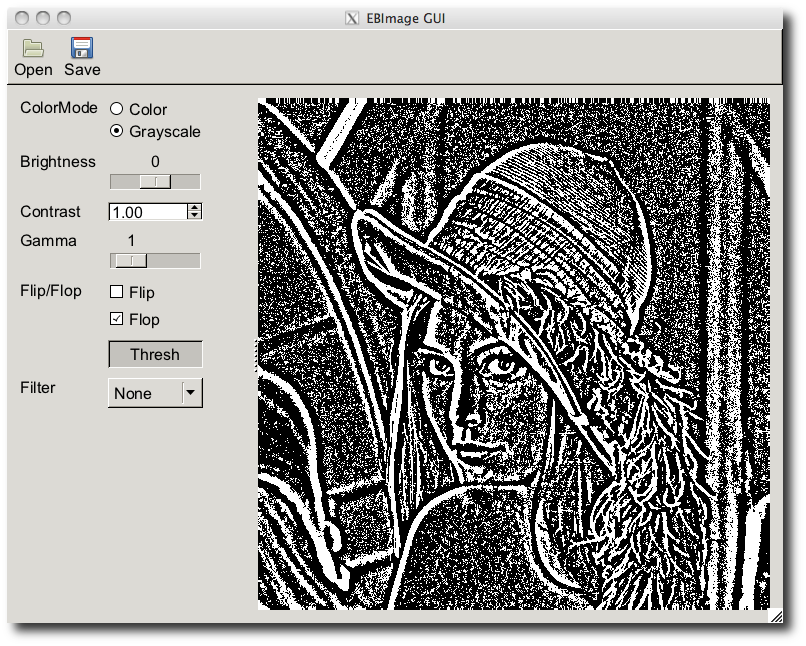
\includegraphics[width=.75\textwidth]{fig-gWidgets-EBImage-gui}
  \caption{A simple GUI for the \pkg{EBImage} package illustrating many selection widgets}
  \label{fig:gWidgets-EBImage-gui}
\end{figure}

This section discusses several such selection controls that serve a
similar purpose but make different use of screen space.

\subsection{Checkbox widget}
\label{sec:gWidgets-checkbox-widget}

The simplest selection control is the \constructor{checkbox} widget
that allows the user to set a state as \code{TRUE} or
\code{FALSE}. The constructor has an argument
\argument{text}{gcheckbox} to set a label and
\argument{checked}{gcheckbox} to indicate if the widget should
initially be checked. The default is \code{TRUE} (there is no third,
uncommitted state as possible in some toolkits). By default the label
will be drawn aside a box which the user can check. If the argument
\argument{use.togglebutton}{gcheckbox} is \code{TRUE}, a toggle button
-- which appears depressed when \code{TRUE} -- is used instead.

In Figure~\ref{fig:gWidgets-EBImage-gui} a toggle button is used for
``Thresh''  and could be constructed as

\begin{Schunk}
\begin{Sinput}
 w <- gwindow("Checkbox example with toggle button")
 cb <- gcheckbox("Thresh", checked=TRUE, use.togglebutton=TRUE,
                 cont=w)
\end{Sinput}
\end{Schunk}

The \method{svalue}{gcheckbox} method returns a logical indicating if
the widget is in the checked state. Use \method{svalue\ASSIGN}{gcheckbox} to set
the state. The label's value is returned by the
\method{[}{gcheckbox} method, and can be adjusted through 
\method{[\ASSIGN}{gcheckbox}. (We take the abstract view that the user
is selecting, or not, from the length-1 vector, so \meth{[} is used to
set the data to select from.)

The default handler would be called on a click event, when the state toggles. If it is desired
that the handler be called only in the \code{TRUE} state, say, one
needs to check within the handler for this. For example
\begin{Schunk}
\begin{Sinput}
 w <- gwindow("checkbox example")
 cb <- gcheckbox("label", cont=w, handler=function(h,...) {
   if(svalue(h$obj))                     # it is checked
     print("define handler here")
 })
\end{Sinput}
\end{Schunk}

\subsection{Radio button widget}
\label{sec:gWidgets-radio-button-widget}

A radio button group allows the user to choose one of a few
items. A radio button group object is returned by
\constructor{gradio}. The items to choose from are specified as a
vector of values to the \argument{items}{gradio} argument (2 or more). These items
may be displayed horizontally or vertically (the default) as specified by the
\argument{horizontal}{gradio} argument which expects a logical. The
\argument{selected}{gradio} argument specifies the initially selected
item, by index,
with a default of the first.


In Figure~\ref{fig:gWidgets-EBImage-gui} a radio button is used for
``ColorMode''  and could be constructed as

\begin{Schunk}
\begin{Sinput}
 w <- gwindow("Radio button example")
 rb <- gradio(c("Color", "Grayscale"), selected=2, 
              horizontal=FALSE, cont=w)
\end{Sinput}
\end{Schunk}


The currently selected item is returned by \method{svalue}{gradio} as
the label text or by the index if the argument \args{index} is
\code{TRUE}. The item may be set with the
\method{svalue\ASSIGN}{gradio} method. Again, the item may be
specified by the label or by an index, the latter when the argument
\code{index=TRUE} is specified. 
\\

The data store is the set of labels and may be respecified with the
\method{[\ASSIGN}{gradio} method.
\\

The handler, if given to the constructor or set with
\meth{addHandlerChanged}, is called on a toggle event.

\subsection{A group of checkboxes}
\label{sec:gWidgets-group-checkboxes}


The group of checkboxes is produced by the
\constructor{gcheckboxgroup} constructor. This convenience widget is
similar to a radio group, only it allows the selection of none, one,
or more than one of a set of items.  The
\argument{items}{gcheckboxgroup} argument is used to specify the
values. The state of whether an item is selected can be set with a
logical vector of the same size as the number of items to the
\argument{checked}{gcheckboxgroup} argument; recycling is used. The
item layout can be controlled by the
\argument{horizontal}{gcheckboxgroup} argument. The default is a
vertical layout (\code{horizontal=FALSE}).


For some toolkits, the argument specification \code{use.table=TRUE}
will render the widget in a table with checkboxes to select from. This
allows much larger sets of items to comfortably be used, as there is a
scrollbar provided. (This provides a similar functionality as using
the \constructor{gtable} widget with multiple selection.)


In Figure~\ref{fig:gWidgets-EBImage-gui} a group of check boxes is
used to allow the user to ``flip'' or ``flop'' the image. It could be
created with

\begin{Schunk}
\begin{Sinput}
 w <- gwindow("Checkbox group example")
 cbg <- gcheckboxgroup(c("Flip","Flop"), horizontal=FALSE, 
                       checked=c(FALSE, TRUE), cont=w)
 
\end{Sinput}
\end{Schunk}
%


The state is retrieved as a character vector through the
\method{svalue}{gcheckboxgroup} method. The \code{index=TRUE} argument
instructs \meth{svalue} to return the selected indices instead. These
are $0$-length if no selection is made. As a checkbox group is like
both a checkbox and a radio button group, one can set the selected
values three different ways. As with a checkbox, the selected values
can be set by specifying a logical vector through the
\method{svalue\ASSIGN}{gcheckboxgroup} method. As with radio button
groups, the selected values can also be set with a character vector
indicating which labels should be selected, or if \code{index=TRUE} is
given, using a numeric index vector.


That is, each of these has the same effect:
\begin{Schunk}
\begin{Sinput}
 svalue(cbg) <- c("Flop")
 svalue(cbg) <- c(FALSE, TRUE)
 svalue(cbg, index=TRUE) <- 2
\end{Sinput}
\end{Schunk}

The labels are returned through the \method{[}{gcheckboxgroup} method
and if the underlying toolkit allows it, set through the
\method{[\ASSIGN}{gcheckboxgroup} method. As with \constructor{gradio},
the \method{length}{gcheckboxgroup} method returns the number of items.

% As an illustration of the related selection widgets, the following
% could be part of a GUI to illustrate densities for various kernels.
% <<>>=
% kerns <- as.character(formals(density.default)$kernel)[-1]

% w <- gwindow("Arguments for density example")
% lyt <- glayout(cont=w)

% lyt[1,1] <- "bw"
% lyt[1,2, anchor=c(-1,0)] <- 
%   gradio(c("nrd0", "nrd", "ucv", "bcv", "SJ"), cont=lyt)

% lyt[2,1] <- "Kernel"
% lyt[2,2, anchor=c(-1,0)] <- gcheckboxgroup(kerns, cont=lyt)

% lyt[3,1] <- "na.rm"
% lyt[3,2, anchor=c(-1,0)] <- 
%   gcheckbox("na.rm", checked=TRUE, use.togglebutton=TRUE, cont=lyt)

% lyt[4,2] <- gbutton("done", cont=lyt, handler=function(h,...) {
%   out <- sapply(1:3, function(i) {
%     widget <- lyt[i,2]
%     svalue(widget)
%   })
%   print(out)                            # make a plot...
% })
% @ 

\subsection{A combo box}
\label{sec:gWidgets-combobox}

Combo boxes are constructed by \constructor{gcombobox}.~\footnote{Some
  make a distinction between drop down lists and combo boxes, the
  latter allowing editing. We don't here, although we note that the
  constructor \constructor{gdroplist} is an alias for
  \code{gcombobox}.}  As with the other selection widgets, the choices
  are specified to the argument \argument{items}{gcombobox}. However,
  this may be a vector of values or a data frame whose first column
  defines the choices. For toolkits which support icons in the combo
  box widget, if the data is specified as a data frame, the second
  column signifies which stock icon is to be used. By design, a third
  column specifies a tooltip to appear when the mouse hovers over a
  possible selection, but this is only implemented for
  \pkg{gWidgetsQt}.

%% ML: this should not be hard to implement with GTK+ 2.12. 
%% JV: hard for me though :( (http://www.daa.com.au/pipermail/pygtk/2009-January/016517.html)

The combo box in Figure~\ref{fig:gWidgets-EBImage-gui} could be coded with:
\begin{Schunk}
\begin{Sinput}
 w <- gwindow("gcombobox example")
 cb <- gcombobox(c("None", "Low", "High"), cont=w)
\end{Sinput}
\end{Schunk}



This example shows how to create a combo box to select from the
available stock icons. For toolkits that support icons in a combo box, they
appear next to the label.
\begin{Schunk}
\begin{Sinput}
 nms <- getStockIcons()                  # gWidgets icons
 d <- data.frame(names=names(nms), icons=names(nms), 
                 stringsAsFactors=FALSE)
 w <- gwindow("Combo box with icons example")
 cb <- gcombobox(d, cont=w)
\end{Sinput}
\end{Schunk}


The argument \argument{editable}{gcombobox} accepts a logical value
indicating if the user can supply their own value by typing into a
text entry area. The default is \code{FALSE}. When editing is
possible, the constructor also has the
\argument{coerce.with}{gcombobox} argument like \code{gedit}.

\paragraph{Methods}
The currently selected value is returned through the
\method{svalue}{gcombobox} method. If \args{index} is \code{TRUE}, the
index of the selected item is given if possible. The value can be set
by its value through the \method{svalue\ASSIGN}{gcombobox} method, or
by index if \args{index} is \code{TRUE}. The \method{[}{gcombobox}
method returns the items of the data store, and
\method{[\ASSIGN}{gcombobox} is used to assign new values to the data
store. The value may be a vector, or data frame if an icon or tooltip
is being assigned. The \method{length}{gcombobox} method returns the
number of possible selections.

The default handler is called when the state of the widget is
changed. This is also aliased to
\method{addHandlerClicked}{gcombobox}. When \code{editable} is
\code{TRUE}, then the \method{addHandlerKeystroke}{gcombobox} method
sets a handler to respond to keystroke events.

\begin{example}{Updating combo boxes}{eg-gWidgets-update-combo}
  A common feature in many GUIs is to have one combo box update
  another once a selection is made. The following employs this to
  create a simple GUI for collecting the arguments for computing the mean of a numeric variable
  (Figure~\ref{fig:gWidgets-mean-default}).
  
  \begin{figure}
    \centering
    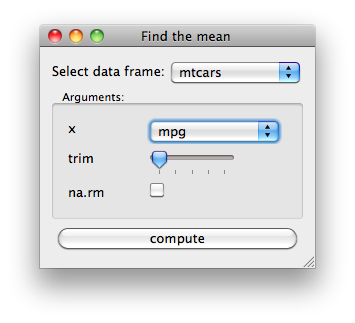
\includegraphics[width=.4\textwidth]{fig-gWidgets-mean-default.png}
    \caption{GUI used to collect arguments for a call to
      \code{mean.default}}
    \label{fig:gWidgets-mean-default}
  \end{figure}
  
  We  make use of the functions from the \pkg{ProgGUIinR} package
  in the following to return character vectors of data frame names and
  numeric variables.

\begin{Schunk}
\begin{Sinput}
 availDfs <- function() {
   c("", ".GlobalEnv", ProgGUIinR:::avail_dfs(.GlobalEnv))
 }
\end{Sinput}
\end{Schunk}
\begin{Schunk}
\begin{Sinput}
 getNumeric <- function(where) {
   val <- get(where, envir=.GlobalEnv)
   ProgGUIinR:::find_vars(val, is.numeric)
 }
\end{Sinput}
\end{Schunk}

Our layout uses nested groups and a \code{glayout} container.
\begin{Schunk}
\begin{Sinput}
 w <- gwindow("Find the mean", visible=FALSE)
 g <- ggroup(cont=w, horizontal=FALSE)
 g1 <- ggroup(cont=g)
 glabel("Select data frame:", cont=g1)
 dfC <- gcombobox(availDfs(), cont=g1)
 ##
 f <- gframe("Arguments:", cont=g, horizontal=FALSE)
 enabled(f) <- FALSE
 lyt <- glayout(cont=f, expand=TRUE)
 l <- list()                             # store widgets
 ##
 lyt[1,1] <- "x"
 lyt[1,2] <- (l$x <- gcombobox("           ", cont=lyt))
 ##
 lyt[2,1] <- "trim"
 lyt[2,2] <- 
   (l$trim <- gslider(from=0, to=0.5, by=0.01, cont=lyt))
 ##
 lyt[3,1] <- "na.rm"
 lyt[3,2] <- 
   (l$na.rm <- gcheckbox("", checked=TRUE, cont=lyt))
 g2 <- ggroup(cont=g)
 compute <- gbutton("compute", cont=g2)
\end{Sinput}
\end{Schunk}

We stored the primary widgets in a list with names matching the
arguments to our function, \function{mean.default}. As well, the
initial argument to the \code{x} combo box pads out the width under
some toolkits.

Here is how we update the \code{x} combo box, when the data frame
combo box is changed. If there is a value, we enable our widgets and
then populate the secondary combo box with the names of the numeric
variables.
\begin{Schunk}
\begin{Sinput}
 addHandlerChanged(dfC, handler=function(h,...) {
   val <- svalue(h$obj)
   enabled(f) <- val !=""
   enabled(compute) <- val != ""
   if(val != "") 
     l$x[] <- getNumeric(val)
   svalue(l$x, index=TRUE) <- 0
 })
\end{Sinput}
\end{Schunk}
%

As we stored the widgets in an appropriately named list, we can
conveniently use \function{do.call} below to write the callback for
the \code{compute} button in just a few lines. The only trick is to
replace the variable name with its actual value.
\begin{Schunk}
\begin{Sinput}
 addHandlerChanged(compute, handler=function(h,...) {
   out <- lapply(l, svalue)
   out$x <- get(out$x, get(svalue(dfC), envir=.GlobalEnv))
   print(do.call(mean.default, out))
 })
\end{Sinput}
\end{Schunk}

\end{example}

%% Removed, above one shows more
% \begin{example}
% <<>>=
% <<echo=FALSE>>=
% require(MASS)
% @   
% <<>>=
% w <- gwindow(visible=FALSE)
% tbl <- glayout(cont=w)
% #
% tbl[1,1] <- "Manufacturer"
% tbl[1,2] <- (man <- 
%          gcombobox(sort(unique(Cars93$Manufacturer)), cont=tbl))
% tbl[2,1] <- "Model"
% tbl[2,2] <- (mod <- gcombobox(c(""), cont=tbl))
% enabled(mod) <- FALSE
% #
% visible(w) <- TRUE
% @ 

% The handler for \code{man} should find the possible models for the
% selected manufacture, then populate \code{mod} with these values for selection.
% <<>>=
% addHandlerChanged(man, handler=function(h,...) {
%   poss <- subset(Cars93, 
%                  subset=Manufacturer == svalue(man), 
%                  select="Model", drop=TRUE)
%   mod[] <- as.character(poss)
%   if(length(poss) == 1)
%     svalue(mod, index=TRUE) <- 1
%   enabled(mod) <- TRUE
% })
% @   
% @   
% \end{example}

\subsection{A slider control}
\label{sec:gWidgets-slider-control}

The \constructor{gslider} constructor creates a scale widget that allows the
user to select a value from the specified sequence.  The basic
arguments mirror that of the \code{seq} function in \R:
\argument{from}{gslider}, \argument{to}{gslider}, and
\argument{by}{gslider}.  However, if \code{from} is a vector, then it is
assumed it presents an orderable sequence of values to select from.
In addition to the arguments to specify the sequence, the argument
\argument{value}{gslider} is used to set the initial value of the
widget and \argument{horizontal}{gslider} controls how the slider is
drawn, \code{TRUE} for horizontal, \code{FALSE} for vertical.

In Figure~\ref{fig:gWidgets-EBImage-gui} a slider is used to update
the brightness. The call is similar to:
\begin{Schunk}
\begin{Sinput}
 w <- gwindow("Slider example")
 brightness <- gslider(from=-1, to=1, by=.05, value=0, 
    handler=function(h,...) {
      cat("Update picture with brightness", svalue(h$obj), "\n")
    }, cont=w)
\end{Sinput}
\end{Schunk}

The \method{svalue}{gslider} method returns the currently chosen
value. The \method{[\ASSIGN}{gslider} method can be used to update the
sequence of values to choose from. 

%% removed this example
% The default handler is called when the slider is changed. Example~\ref{ex-gWidgets-sliders-spinbuttons}
% shows how this can be used to update a graphic.

In Figure~\ref{fig:gWidgets-EBImage-gui} the \pkg{gWidgetsRGtk2}
package is used. This toolkit shows a tip with the current value, for
others the slider implementation does not show the value. One can
add a label to show this (or combine the slider with a spin
button). Adding a label follows this pattern:

\begin{Schunk}
\begin{Sinput}
 w <- gwindow("Add a label to the slider", visible=FALSE)
 g <- ggroup(cont=w, expand=TRUE)
 sl <- gslider(from=0, to=100, by=1, cont=g, expand=TRUE)
 l <- glabel(sprintf("%3d", svalue(sl)), cont=g)
 font(l) <- c(family="monospace")
 addHandlerChanged(sl, function(h,...) {
   svalue(h$action) <- sprintf("%3d", svalue(h$obj))
   }, action=l)
 visible(w) <- TRUE
\end{Sinput}
\end{Schunk}
(Using \code{sprintf} and \code{monospace} ensures the label takes a
fixed amount of space.)


\subsection{A spin button control}
\label{sec:gWidgets-spin-button-control}

The spin button control constructed by \constructor{gspinbutton} is
similar to \constructor{gslider} when used with numeric data, but
presents the user a more precise way to select the value. The
\code{from}, \code{to} and \code{by} arguments must be specified. The
argument \argument{digits}{gspinbutton} specifies how many digits are
displayed.

In Figure~\ref{fig:gWidgets-EBImage-gui} a spin button is used to
adjust the contrast, a numeric value. The following will reproduce it

\begin{Schunk}
\begin{Sinput}
 w <- gwindow("Spin button example")
 sp <- gspinbutton(from=0, to=10, by=.05, value=1, cont=w)
\end{Sinput}
\end{Schunk}


% \begin{example}{Example of sliders and spin buttons}{ex-gWidgets-sliders-spinbuttons}
%   The use of sliders and spin buttons to dynamically adjust a graphic
%   is common in \R\/ GUIs targeted towards teaching statistics. Here is
%   an example, similar to the \code{tkdensity} example of \pkg{tcltk},
%   where the slider controls the bandwidth of a density estimation and
%   the spin button the sample size of a random sample.
% <<results=hide>>=  
% w <- gwindow("Slider and Spin Button example") 
% tbl <- glayout(cont=w)
% tbl[1,1] <- "sample size"
% tbl[1,2] <- (spinner <- gspinbutton(from=10, to=100, by=5, 
%                                     value=25, cont=tbl))
% tbl[2,1] <- "adjusted bandwidth"
% tbl[2,2, expand=TRUE] <- (slider <- gslider(from=0.1, to=1, 
%            by=0.01, value=1, cont=tbl))

% plotGraph <- function(h,...) {
%   x <- rexp(svalue(spinner))
%   plot(density(x, adj=svalue(slider)))
% }
% sapply(list(spinner, slider), function(i) 
%   addHandlerChanged(i, handler=plotGraph))
% @ 
% \end{example}




\subsection{Selecting from the file system}
\label{sec:gWidgets-selecting-from-file}

The \constructor{gfile} dialog allows one to select a file or directory
from the file system. This is a modal dialog, which returns the name
of the selected file or directory. The \constructor{gfilebrowse}
constructor creates a widget that has a button that
initiates this selection.  

The ``Open'' button in Figure~\ref{fig:gWidgets-EBImage-gui} is bound
to this action:


\begin{Schunk}
\begin{Sinput}
 f <- gfile("Open an image file",
            type="open",
            filter=list("Image file"=list(
                          patterns=c("*.gif", "*.jpeg", "*.png")
                          ),
              "All files" = list(patterns = c("*"))
              ))
 if(!is.na(f)) 
   readImage(f) ## ...
\end{Sinput}
\end{Schunk}


The selection type is specified by the \code{type} argument with
values of \code{open}, to select an existing file; \code{save} to
select a file to write to; and \code{selectdir} to select a
directory. The \argument{filter}{gfile} argument is toolkit
dependent. For \code{RGtk2}, the \argument{filter}{gfile} argument
used above will filter the possible selections. The dialog returns
the path of the file, or \code{NA} if the dialog was canceled.

Although working with the return value is easy enough, if desired, one can specify a
handler to the constructor to call on the file or directory name. The
component \code{file} of the first argument to the handler contains
the file name.


% <<eval=FALSE>>=
% if(!is.na(tmp <- gfile())) 
%   source(tmp)
% ## or
% gfile(handler=function(h,...) {
%   if(!is.na(h$file))
%     source(h$file) 
% })   
% @ 
% %$


\subsection{Selecting a date}
\label{sec:gWidgets-selecting-date}

The \constructor{gcalendar} constructor returns a widget for selecting
a date. If there is a native widget in the underlying toolkit, this
will be a text area with a button to open a date selection
widget. Otherwise it is just a text entry widget.  The argument
\argument{text}{gcalendar} argument specifies the initial text. The
format of the date is specified by the \argument{format}{gcalendar}
argument.

The methods for the widget inherit from \code{gedit}. In particular,
the \method{svalue}{gcalendar} method returns the text in the text box
as a character vector formatted by the value specified by the
\argument{format}{gcalendar} argument. To return a value of a
different class, pass a function, such as \code{as.Date} to the
\argument{coerce.with}{gcalendar} argument.



\begin{example}{Selecting from a file system}{eg-gwidgets-file-system-II}
%% REturn to file system search

\begin{figure}
  \centering
  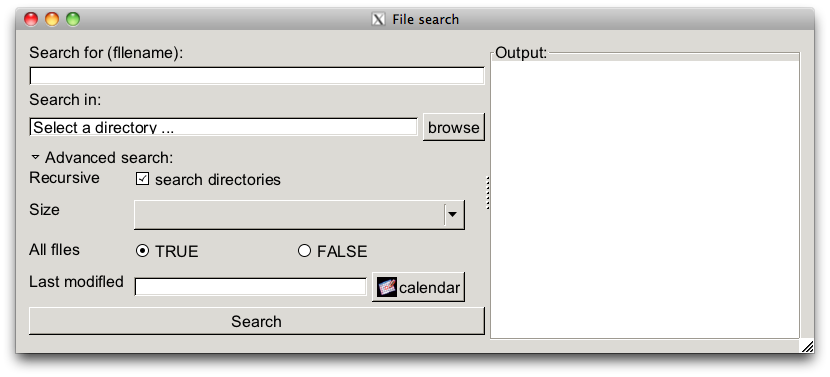
\includegraphics[width=.8\textwidth]{fig-gWidgets-file-search-advanced.png}
  \caption{File search dialog showing advanced search features disclosed}
  \label{fig:file-search-advanced}
\end{figure}

We return to the File selection GUI used as an example in
Chapter~\ref{sec:overview}. Our goal here is to add in more features
to have advanced searching. Imagine we have a function \code{file\_search} which in
addition to arguments for  a pattern and directory has arguments
\code{modified} to pass a date string, \code{size} to pass a
descriptive \code{small}, \code{medium} or \code{large} and an
argument \code{visible} to indicate if all files (including dot files)
should be looked at. 

We want to update our GUI to collect values for these.
Since these are advanced options, we want the user to have access only
on request. We use \code{gexpandgroup} to provide this. Here we define
the additional code for the layout:


\begin{Schunk}
\begin{Sinput}
 advSearch <- gexpandgroup("Advanced search:", cont=f)
 visible(advSearch) <- FALSE
 tbl <- glayout(cont=advSearch)
 tbl[1,1] <- "Recursive"
 tbl[1,2] <- (advRec <- 
    gcheckbox("search directories", checked=TRUE, cont=tbl))
 tbl[2,1] <- "Size"
 tbl[2,2] <- (advSize <- 
    gcombobox(c("", "small", "medium", "large"),  cont=tbl))
 tbl[3,1] <- "All files"
 tbl[3,2] <- (advVisible <- 
    gradio(c(TRUE, FALSE), horizontal=TRUE, cont=tbl))
 tbl[4,1] <- "Last modified"
 tbl[4,2] <- (advModified <- 
              gcalendar("", format="%Y-%m-%d", cont=tbl))
\end{Sinput}
\end{Schunk}

As can be seen (Figure~\ref{fig:file-search-advanced}), we use a grid
layout and a mix of the controls offered by \pkg{gWidgets}.



We need to modify our button handler so that it uses these values, if
specified. We only do so if this part of the GUI is disclosed, by
checking the output of \code{visible(advSearch)}.

\begin{Schunk}
\begin{Sinput}
 addHandlerChanged(searchBtn, handler=function(h,...) {
   pattern <- glob2rx(svalue(txtPattern))
   start_dir <- svalue(startDir)
   subfolders <- TRUE
   modified <- NULL
   size <- NULL
   visible <- TRUE
 
   ## new
   if(visible(advSearch)) {
     subfolders <- svalue(advRec)
     if((tmp <- svalue(advSize)) != "") size <- tmp
     visible <- svalue(advVisible)
     if(!is.na(tmp <- svalue(advModified))) modified <- tmp
   }
   
   ## function call
   fnames <- file_search(pattern, start_dir, subfolders, 
                         modified=modified,
                         size=size, visible=visible)
   dispose(searchResults)                # clear
   if(length(fnames))
     svalue(searchResults) <- fnames
   else
     galert("No matching files found", parent=w)
 })
\end{Sinput}
\end{Schunk}




\end{example}


\section{Display of tabular data}
\label{sec:gWidgets-tabular-data-display}


The \constructor{gtable} constructor~\footnote{The
  \constructor{gtable} widget shows clearly the trade offs between
  using \pkg{gWidgets} and a native toolkit under \R. As will be seen
  in later chapters, setting up a table to display a data frame using
  the toolkit packages directly can involve a fair amount of coding as
  compared to \constructor{gtable}, which makes it very easy. However,
  \pkg{gWidgets} provides far less functionality. For example, there
  is no means to adjust the formatting of the displayed text, or to
  embed other widgets into the tabular display, such as check boxes.
} produces a widget that displays data in a tabular form from which
the user can select one (or more) rows. The widgets performance under
\pkg{gWidgetsRGtk2} and \pkg{gWidgetsQt} is much faster and able to
handle larger data stores
%% ML: I'm assuming gWidgetsQt will soon take advantage of the DataFrameModel
than under \pkg{gWidgetstcltk}, as there is no native table widget in
\tcltk. At a minimum, all perform well on moderate-sized data sets (10
or so columns and fewer than 500 rows).~\footnote{For
  \pkg{gWidgetsRGtk2}, the \constructor{gdfedit} widget can show very
  large tables taking advantage of the underlying \pkg{RGtk2Extras}
  package. For \pkg{gWidgetsQt} the constructor
  \constructor{gbigtable} can be used to show very large tables.}

The data is specified through the \argument{items}{gtable}
argument. This value may be a data frame, matrix or vector. Vectors and
matrices are coerced to data frames, with
\code{stringsAsFactors=FALSE}.  The data is presented in a tabular
form, with column headers derived from the \code{names} attribute of
the data frame (but no row names). The \argument{items}{gtable}
argument can be a $0$-length data frame, but the column classes must
match the eventual data to be used.


To illustrate, a widget to select from the available data frames in
the global environment can be generated with
\begin{Schunk}
\begin{Sinput}
 w <- gwindow("gtable example")
 dfs <- gtable(ProgGUIinR:::avail_dfs(), cont=w)
\end{Sinput}
\end{Schunk}

%% sizes
Often the table widget is added to a box container with the argument
\code{expand=TRUE}. Otherwise, the size of the widget should be specified
through \meth{size\ASSIGN}. This size can be list with components \code{width}
and \code{height} (pixel widths). As well, the component
\code{columnWidths} can be used to specify the column
widths. (Otherwise a heuristic is employed.)

\paragraph{Icons}
The \argument{icon.FUN}{gtable} argument can be used to place a stock
icon in a left-most column.  This argument takes a function of a
single argument -- the data frame being shown -- and should return a
character vector of stock icon names, one for each row.

\paragraph{Selection}
Users can select by case (row) -- not by observation (column) -- from
this widget. The actual value returned by a selection is controlled by
the constructor's argument \argument{chosencol}{gtable}, which
specifies which column's value will be returned for the given index,
as the user can only specify the row. The \argument{multiple}{gtable}
argument can be specified to allow the user to select more than one
row.

\paragraph{Methods}
The \method{svalue}{gtable} method will return the currently selected
value. If the argument \code{index} is specified as \code{TRUE}, then
the selected row index (or indices) will be returned. These refer to
the data store, not the visible data when filtering is being used (below). The
argument \code{drop} specifies if just the chosen column's value is
returned (the default) or, if specified as \code{FALSE}, the entire row.
 
The underlying data store is referenced by the \method{[}{gtable}
method. Indices may be used to access a slice. Values may be set using
the \method{[\ASSIGN}{gtable} method, but be warned it is not as
flexible as assigning to a data frame. The underlying toolkits may not
like to change the type of data displayed in a column or reduce the
number of columns displayed, so when updating a column do not assume
some underlying coercion, as is done with \R's data frames. (This is
why the initial items, even if a $0$-length data frame, need to be of
the correct class.) To replace the data store, the \code{[\ASSIGN} can
be used, as with \code{obj[] \ASSIGN\/ new\_data\_frame}. The methods
\method{names}{gtable} and \method{names\ASSIGN}{gtable} refer to the
column headers, and \method{dim}{gtable} and \method{length}{gtable}
the underlying dimensions of the data store.

To update the list of data frames in our \code{dfs} widget, one can define a function such as
\begin{Schunk}
\begin{Sinput}
 updateDfs <- function() {
   dfs[] <- ProgGUIinR:::avail_dfs()
 }
\end{Sinput}
\end{Schunk}


\paragraph{Handlers}
Selection is done through a single click. The \method{addHandlerClick}{gtable}
method  can be used to assign a handler to those events. The default
handler, \method{addHandlerDoubleclick}{gtable}, will assign a
handler for a double click event. Also of interest are the
\method{addHandlerRightclick}{gtable} and
\method{add3rdMousePopupMenu}{gtable} methods for assigning handlers
to right-click events.


To add a handler to the data frame selection widget above, we could have:
\begin{Schunk}
\begin{Sinput}
 addHandlerDoubleclick(dfs, handler=function(h,...) {
   val <- svalue(h$obj)
   print(summary(get(val, envir=.GlobalEnv))) # some action
 
 })
\end{Sinput}
\end{Schunk}

%% Factor example
\begin{example}{Collapsing factors}{eg:gWidgets-collapse-factor}
 
  \begin{figure}
    \centering
    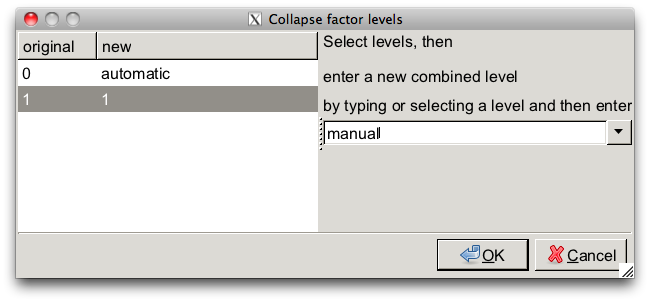
\includegraphics[width=.8\textwidth]{fig-gWidgets-collapse-factor.png}
    \caption{A GUI to facilitate the recoding or a factor's levels. For this, one selects the desired levels to rename or collapse, then enters a new label on the right. Activating the combo box will update the "new" column on the left.}
    \label{fig:gWidgets-collapse-factor}
  \end{figure}
  
  
  
  A somewhat tedious task in \R{} is the recoding or collapsing of
  factor levels. This example provides a GUI to facilitate this. In
  Section~\ref{sec:modal-window} we provided a function to wrap this
  GUI within a modal dialog. Here we just setup the GUI. 
  
  We will use a reference class, as it allows us to couple together
  the main method and the widgets without needing to worry about
  scoping issues. For formatting purposes, we define the methods
  individually, then piece together.
  
  Our initialization call simple stores the values and then passes on
  the call to make the GUI.
\begin{Schunk}
\begin{Sinput}
 initialize <- function(f, cont=gwindow()) {
   old <<- as.character(f)
   make_gui(cont)
   callSuper()
 }
\end{Sinput}
\end{Schunk}

This \code{make\_gui} function does the hard
work. (Figure~\ref{fig:gWidgets-collapse-factor} shows a screenshot.)
We have just two widget, placed in a paned group. The left one is a
table that displays two columns. The first to list the old values, the
second to list the collapsed or recoded values. The right one is a
combo box that allows one to enter a new factor level or select a
current one. The handler on the combo box updates the second column of
the table to reflect the new values. We block any handler calls to
avoid a loop when we set the index back to 0.
\begin{Schunk}
\begin{Sinput}
 make_gui <- function(cont) {
   g <- gpanedgroup(cont=cont)
   levs <- sort(unique(as.character(old)))
   d <- data.frame(original=levs,
                   new=levs, stringsAsFactors=FALSE)
   #
   widget <<- tbl <- gtable(d, cont=g,  multiple=TRUE)
   size(tbl) <- c(300, 200)
   #
   g1 <- ggroup(cont=g, horizontal=FALSE)
   instructions <- gettext("Select levels, then\n 
 enter a new combined level\n
 by typing or selecting a level and then enter")
   #
   glabel(instructions, cont=g1)
   cb <- gcombobox(levs, selected=0, editable=TRUE, cont=g1)
   enabled(cb) <- FALSE
   #
   addHandlerClicked(widget, function(h,...) {
     ind <- svalue(widget, index=TRUE)
     enabled(cb) <- (length(ind) > 0)
   })
   
   addHandlerChanged(cb, handler=function(h,...) {
     ind <- svalue(tbl, index=TRUE)
     if(length(ind) == 0) 
       return()
     #
     tbl[ind,2] <- svalue(cb)
     svalue(tbl, index=TRUE) <- 0
     blockHandler(cb)
     cb[] <- sort(unique(tbl[,2]))
     svalue(cb, index=TRUE) <- 0
     unblockHandler(cb)
   })
 }
\end{Sinput}
\end{Schunk}

This method returns the newly recoded factor. The tediousness of the task
is in the specification of the new levels, not necessarily this. 
\begin{Schunk}
\begin{Sinput}
 get_value <- function() {
   "Return factor with new levels"
   old_levels <- widget[,1]
   new_levels <- widget[,2]
   new <- old
   for(i in seq_along(old_levels)) # one pass
     new[new == old_levels[i]] <- new_levels[i]
   factor(new)
 }
\end{Sinput}
\end{Schunk}
%

Finally, we stitch the above together into a reference class.
\begin{Schunk}
\begin{Sinput}
 CollapseFactor <- setRefClass("CollapseFactor",
                               fields=list(
                                old="ANY",
                                widget="ANY"
                                ),
                              methods=list(
                                initialize=initialize,
                                make_gui = make_gui,
                                get_value=get_value
                              ))
\end{Sinput}
\end{Schunk}


  
\end{example}


\paragraph{Filtering}
The arguments \argument{filter.column}{gtable} and
\argument{filter.FUN}{gtable} allow one to specify whether the user
can filter, or limit, the display of the values in the data store. The
simplest case is if a column number is specified to the
\code{filter.column} argument. In which case a combo box is added to
the widget with values taken from the unique values in the specified
column. Changing the value of the combo box restricts the display of
the data to just those rows where the value in the filter column
matches the combo box value. More advanced filtering can be specified
using the \argument{filter.FUN}{gtable} argument. If this is a
function, then it takes arguments \code{(data\_frame, filter.by)}
where the data frame is the data, and the \code{filter.by} value is
the state of a combo box whose values are specified through the
argument \argument{filter.labels}{gtable}. This function should return
a logical vector with length matching the number of rows in the data
frame.  Only rows corresponding to \code{TRUE} values will be
displayed. 


If \code{filter.FUN} is the character string ``\code{manual}'' then
the \method{visible\ASSIGN}{gtable} method can be used to control the
filtering, again by specifying a logical vector of the proper
length. See Example~\ref{ex-gWidgets-filter-gtable} for an
application.



\begin{example}{Simple filtering}{ex-gWidgets-simple-filter-gtable}
  We use the \code{Cars93} data set from the \pkg{MASS} package to
  show how to set up a display of the data which provides simple
  filtering based on the type of car, whose value is stored in column 3.
  
\begin{Schunk}
\begin{Sinput}
 require(MASS)
 w <- gwindow("gtable example")
 tbl <- gtable(Cars93, chosencol=1, filter.column=3, cont=w)
\end{Sinput}
\end{Schunk}

Adding a handler for the double click event is illustrated below. This
handler prints both the manufacturer and the model of the currently
selected row when called.
\begin{Schunk}
\begin{Sinput}
 addHandlerChanged(tbl, handler=function(h,...) {
   val <- svalue(h$obj, drop=FALSE)
   cat(sprintf("You selected the %s %s", val[,1], val[,2]))
 })
\end{Sinput}
\end{Schunk}
%%$ emacs
\end{example}


\begin{example}{More complex filtering}{ex-gWidgets-filter-gtable}
%% Example of hand-built filter using gtable

\begin{figure}
  \centering
  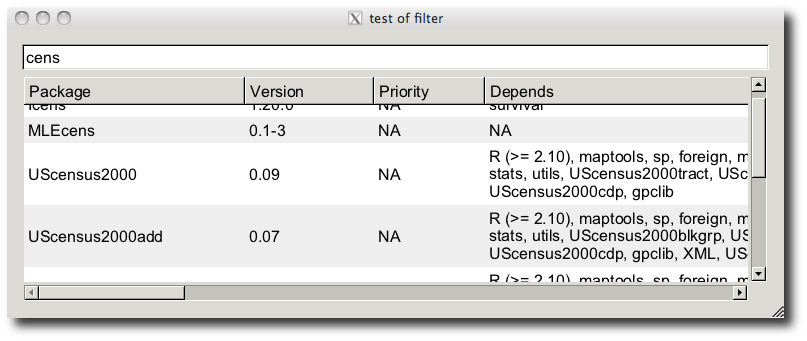
\includegraphics[width=.8\textwidth]{fig-gWidgets-filter-example}
  \caption{Example of using a filter to narrow the display of tabular data}
  \label{fig:gWidgets-filter-example}
\end{figure}

Even with moderate-sized data sets, the number of rows can be quite large, in which case it is
inconvenient to use a table for selection unless some means of searching or filtering the
data is used. This example uses the many possible CRAN packages, to show how a
\code{gedit} instance can be used as a search box to filter the display of
data (Figure~\ref{fig:gWidgets-filter-example}). The \code{addHandlerKeystroke} method is used so that the search
results are updated as the user types.


The \code{available.packages} function returns a data frame of all
available packages. If a CRAN site is not set, the user will be
queried to set one.
\begin{Schunk}
\begin{Sinput}
 ap <- available.packages()       # pick a cran site
\end{Sinput}
\end{Schunk}

This basic GUI is barebones, for example we skip adding text labels to guide the user. 
\begin{Schunk}
\begin{Sinput}
 w <- gwindow("test of filter")
 g <- ggroup(cont=w, horizontal=FALSE)
 ed <- gedit("", cont=g)
 tbl <- gtable(ap, cont=g, filter.FUN="manual", expand=TRUE)
\end{Sinput}
\end{Schunk}
The \argument{filter.FUN}{gtable} value of \qcode{manual} allows us to
filter by specifying a logical vector.

Different search criteria may be desired, so it makes sense to
separate out this code from the GUI code using a function. The one below
uses \code{grep} to match, so that regular expressions can be
used. Another reasonable choice would be to use the first letter of
the package. (That filtering could also be specified easily through the
\argument{filter.FUN}{gtable} argument.)

\begin{Schunk}
\begin{Sinput}
 ourMatch <- function(curVal, vals) {
   grepl(curVal, vals)
 }
\end{Sinput}
\end{Schunk}

Finally, the \code{addHandlerKeystroke} method calls its handler
every time a key is released while the focus is in the edit widget. In
this case, the handler finds the matching indices using the
\code{ourMatch} function, converts these into logical format, and then
updates the display using the \meth{visible\ASSIGN} method for
  \code{gtable}.
\begin{Schunk}
\begin{Sinput}
 id <- addHandlerKeystroke(ed, handler=function(h, ...) {
   vals <- tbl[, 1, drop=TRUE]
   curVal <- svalue(h$obj)
   vis <- ourMatch(curVal, vals)
   visible(tbl) <- vis
 })
\end{Sinput}
\end{Schunk}
\end{example}


\begin{example}{Using the ``observer pattern'' to write a workspace view}{ex-gWidgets-ws-browser}
% XXX Tighten up -- use Observer/obsrevable not MVC
% XXX Add UML diagram
% Head First Design Patterns
% By: Eric T Freeman; Elisabeth Robson; Bert Bates; Kathy Sierra
% Publisher: O'Reilly Media, Inc.
% Pub. Date: October 25, 2004


\begin{figure}
  \centering
  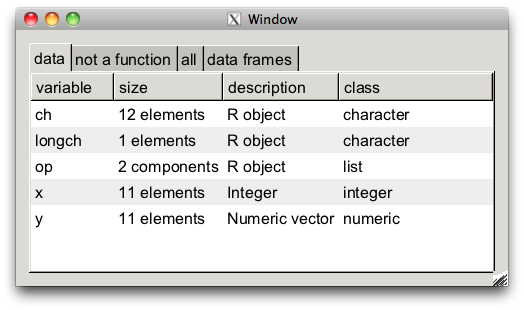
\includegraphics[width=.6\textwidth]{fig-gWidgets-ws-browser.png}
  \caption{A notebook showing various views of the objects in the global workspace. The example uses the Observer pattern to keep the views synchronized.}
  \label{fig:gWidgets-ws-browser}
\end{figure}


This example takes the long way to make a workspace browser. (The
short way is to use \constructor{gvarbrowser}.) The goal is to produce
a GUI that will allow the user to view the objects in their current
workspace. We would like these views to be dynamic though -- when the
workspace changes we would like the views to update. Furthermore, we
may want to have different views, such as one for functions and one
for data sets.

This pattern where a central, dynamic source of data is to used and
shared amongst many different pieces of a GUI is a common one. To
address the complexity that arises as the components of a GUI get more
intertwined, standard design patterns have been employed. For this
task, the \defn{Observer Pattern} is often used. This pattern is
defined in~\footcite{head-first-design-patterns} to describe a
one-to-many relationship between a set of objects where when the state
of one object changes, all of its dependents are notified.

% %% http://yuml.me/diagram/scruffy/usecase/Observable|add_observer();remove_observer();notify_observers().
% %% http://yuml.me/diagram/scruffy/usecase/Observer| update().
% \begin{figure}
%   \centering
%   \includegraphics[width=.35\textwidth]{fig-gWidgets-observable.png}
%   \includegraphics[width=.35\textwidth]{fig-gWidgets-observer.png}
%   \caption{Observable and Observer classes and their basic methods. An
%     observable object may have many observers which are notified
%     through their update method when a change is made.}
%   \label{fig:observer-observable}
% \end{figure}



Figure~\ref{fig:observer-observable} shows a class diagram of the two
different types of objects involved:
\begin{description}
\item[Observables] The objects which notify observers when a change is
  made. The basic methods are to add and remove an observer; and to
  notify all observers when a change is made. In our example, we will
  create a workspace model which will notify the various observers
  (views) when \R's global workspace has changes.
\item[Observers] The objects which listen for changes to the
  observable object. Observers are registered with the observable and
  are notified of changes by a call to the observer's \code{update}
  method. In our example, the different views of the workspace are
  observers.
\end{description}

An implementation of the observable class using reference classes
follows. The different observers are stored in a list.

\begin{Schunk}
\begin{Sinput}
 setRefClass("Observable",
             fields=list(observers="list"),
             methods=list(
               add_observer=function(o) {
                 "Add an observer."
                 observers <<- c(observers, o)
               },
               remove_observer=function(o) {
                 "Remove observer"
                 ind <- sapply(observers, identical, y=o)
                 if(any(ind)) 
                   observers[[which(ind)]] <<- NULL
                 
               },
               notify_observers=function(...) {
                 "Notify observers there has been a change"
                 sapply(observers, function(o)
                        o$update(.self, ...))
               }))
 
\end{Sinput}
\end{Schunk}
%
This can get more involved (we implement signals or we could allow
observers to be blocked, etc.), but we keep
it simple for this example. 


\begin{figure}
  \centering
  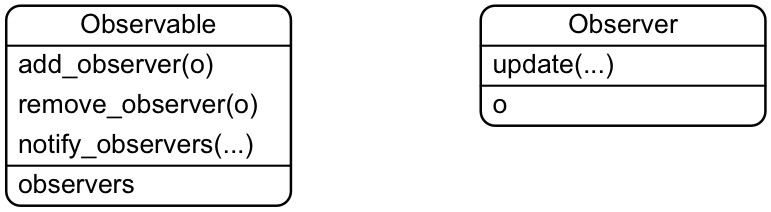
\includegraphics[width=.6\textwidth]{fig-gWidgets-observable-observer-uml.png}
 \caption{Observable and Observer classes and their basic methods. An observable object may have many observers which are notified through their update method when a change is made.}
  \label{fig:observer-observable}
\end{figure}

The basic observer pattern just creates a class for observers so that
they have an \meth{update} method. Again, a simple implementation
follows:


\begin{Schunk}
\begin{Sinput}
 setRefClass("Observer",
       fields=list(o = "function"),
       methods=list(
         update=function(...) {
           "Call self. Arguments passed by notify_observers"
           o(.self, ...)
         }))
\end{Sinput}
\end{Schunk}
%

A model is an observable with properties. When these properties are
changed, any observers are notified. Our workspace will be stored in a
model instance.  Models generally have getter and setter methods for
these properties. The setter method would typically store a value and
then notify any observers of the model.

As an example, we define this subclass:
\begin{Schunk}
\begin{Sinput}
 setRefClass("Model",
       contains="Observable",
       methods=list(
         get=function(key) {
           "get value of property"
           base:::get(key)
         },
         set=function(key, value, notify=TRUE) {
           "Set key field to value. Notify observers."
           assign(key, value, inherits=TRUE)
           if(notify)
             notify_observers(model=.self)
           invisible()
         }))
\end{Sinput}
\end{Schunk}
%



To illustrate how this works, we define a simple subclass of our
\class{Model} call and an observer.
\begin{Schunk}
\begin{Sinput}
 TestModel <- setRefClass("TestModel",
                          contains="Model",
                          fields=list(prop1="character"))
 m <- TestModel$new()
 f <- function(model,...) print(model$get("prop1"))
 o <- getRefClass("Observer")$new(o=f)
 m$set("prop1", "Some value")
 m$add_observer(o)
 m$set("prop1", "A new value")           # now f is called
\end{Sinput}
\begin{Soutput}
[1] "A new value"
\end{Soutput}
\end{Schunk}



The data in our workspace model keeps track of the objects in the
workspace by name and a digest of each variable. The digest allows us
to compare if objects have been updated, not just renamed. As
notifying views can be potentially expensive, we will only notify on a
change.

\begin{Schunk}
\begin{Sinput}
 WSModel <- setRefClass("WSModel",
                        contains="Observable",
                        fields=list(
                          ws_objects="character",
                          ws_objects_digest="character"
                          ))
\end{Sinput}
\end{Schunk}
%

For the task at hand, we don't really have a \code{set} method, but
rather we define a \code{refresh} method to synchronize the workspace
with our model object. We then notify observers if there is a
change. This model needs to track changes in the underlying
workspace. This can be done calling the \code{refresh} method at
periodic intervals, through a \code{taskCallback}, or by user request.

\begin{Schunk}
\begin{Sinput}
 require(digest)
 WSModel$methods(refresh = function() {
   "refresh vector of ws_objects if applicable"
   x <- sort(ls(envir=.GlobalEnv))
   ## filter out envRefClass objects --
   isRef <- function(i) 
     is(get(i, envir=.GlobalEnv), "envRefClass")
   ind <- sapply(mget(x, .GlobalEnv), is, class2="envRefClass")
   x <- x[!ind]
   ds <- sapply(mget(x,envir=.GlobalEnv), digest)
   
   if((length(ds) != length(ws_objects_digest)) ||
      length(ws_objects_digest) == 0 ||
      any(ds != ws_objects_digest)) {
     ws_objects <<- x
     ws_objects_digest <<- ds 
     notify_observers()
   }
   invisible()
 })
\end{Sinput}
\end{Schunk}
%
The \code{get\_objects} method, which returns the names of the
objects in the work space,  adds some complexity, but allows us to
filter by class.

As can be seen we pass in the model to the observers. We need a
standard interface for getting the data from the model, so define a
\code{get} method. We add an additional argument, \code{klass}, to
filter by class.

\begin{Schunk}
\begin{Sinput}
 WSModel$methods(get = function(klass) {
   "Get objects. If klass given, restrict to those. 
 Klass may have ! in front, as in '!function'"
   if(missing(klass) || length(klass) == 0)
     return(ws_objects)
   #
   ind <- sapply(mget(ws_objects, .GlobalEnv), function(x) {
     any(sapply(klass, function(j)  {
       if(grepl("^!", j))
         !is(x, substr(j, 2, nchar(j)))
       else
         is(x, j)
     }))
   })
   #
   if(length(ind))
     ws_objects[ind]
   else
     character(0)
 })
\end{Sinput}
\end{Schunk}
%



To use this model, we create a base view class adding a new method to
set the model. One could store a reference to the model in the view --
which makes it easier to remove a model -- but keep it simple here.
\begin{Schunk}
\begin{Sinput}
 setRefClass("WSView",
             contains="Observer",
             methods=list(
               set_model=function(model) {
                 "Add view as observer"
                 model$add_observer(.self)
               }
               ))
\end{Sinput}
\end{Schunk}
%

The following \class{WidgetView} class uses the template method
pattern leaving subclasses to construct the widgets through the call
to \meth{initialize}. 

\begin{Schunk}
\begin{Sinput}
 WidgetView <- 
   setRefClass("WidgetView",
               contains="WSView",
               fields=list(
                 klass="character", # which classes to show
                 widget = "ANY"
                 ),
               methods=list(
                 initialize=function(parent, model, ...) {
                   if(!missing(model)) set_model(model)
                   if(!missing(parent)) init_widget(parent, ...)
                   initFields()
                   .self
                 },
                 init_widget=function(parent, ...) {
                   "Initialize widget"
                 }))
\end{Sinput}
\end{Schunk}
% 


%

We write a \class{WidgetView} subclass to view the workspace
objects using a \code{gtable} widget.
\begin{Schunk}
\begin{Sinput}
 TableView <-
   setRefClass("TableView",
         contains="WidgetView",
         methods=list(
           init_widget=function(parent, ...) {
             widget <<- gtable(makeDataFrame(character(0)),
                               cont=parent, ...)
           },
           update=function(model, ...) {
             widget[] <<- makeDataFrame(model$get(klass))
           }))
\end{Sinput}
\end{Schunk}
%


This subclass of the widget view class shows
the values in the workspace using a table widget. The
\code{makeDataFrame} function generates the details. We now turn to
the task of defining that function.

To generate data on each object, we define some S3 classes. These are
more convenient than reference classes for this task. First we want a
nice description of the size of the object:
\begin{Schunk}
\begin{Sinput}
 sizeOf <- function(x, ...) UseMethod("sizeOf")
 sizeOf.default <- function(x, ...) "NA"
 sizeOf.character <- sizeOf.numeric <- 
   function(x, ...) sprintf("%s elements", length(x))
 sizeOf.matrix <- function(x, ...) 
   sprintf("%s x %s", nrow(x), ncol(x))
\end{Sinput}
\end{Schunk}

%

Now, we desire a short description of the type of object we have.
\begin{Schunk}
\begin{Sinput}
 shortDescription <- function(x, ...) 
   UseMethod("shortDescription")
 shortDescription.default <- function(x, ...) "R object"
 shortDescription.numeric <- function(x, ...) "Numeric vector"
 shortDescription.integer <- function(x, ...) "Integer"
\end{Sinput}
\end{Schunk}
%

The following function produces a data frame summarizing the objects passed in
by name to \code{x}. It is a bit awkward, as the data comes row by
row, not column by column and we want to have a default when \code{x}
is empty.
\begin{Schunk}
\begin{Sinput}
 makeDataFrame <- function(x, envir=.GlobalEnv) {
   d <- data.frame(variable=character(0),
                   size=character(0), description=character(0), 
                   class=character(0),
                   stringsAsFactors=FALSE)
   if(length(x)) {
     l <- mget(x, envir)
     d <- data.frame(variable=x,
                     size=sapply(l, sizeOf),
                     description=sapply(l, shortDescription),
                     class = sapply(l, function(i) class(i)[1]),
                     stringsAsFactors=FALSE)
   }
   d
 }
\end{Sinput}
\end{Schunk}

To illustrate the flexibility of this framework, we also define a
subclass of \code{WidgetView} to show just the data frames in a combo
box. Selecting a data frame is a common task in R GUIs, and this
allows keeps the selection up to date.

\begin{Schunk}
\begin{Sinput}
 DfView <-
   setRefClass("DfView",
         contains="WidgetView",
         methods=list(
           initFields = function(...) klass <<- "data.frame", 
           init_widget = function(parent, ...) {
             d <- data.frame("Data frames"=character(0),
                             stringsAsFactors=FALSE)
             widget <<- gcombobox(d, cont=parent, ...)
           },
           update = function(model, ...) {
             widget[] <<- model$get(klass)
           }
           ))
\end{Sinput}
\end{Schunk}
%

We can put these pieces together to make a simple GUI. 
\begin{Schunk}
\begin{Sinput}
 w <- gwindow()
 nb <- gnotebook(cont=w)
 #
 model <- getRefClass("WSModel")$new()
 #
 view <- TableView$new(parent=nb, model=model, label="data")
 view$klass <- c("factor", "numeric", "character", 
                 "data.frame", "matrix", "list")
 #
 view1 <- TableView$new(parent=nb, model=model, 
                        label="not a function")
 view1$klass <- "!function"
 #
 view2 <- TableView$new(parent=nb, model=model, label="all")
 ## a bit contrived here
 view3 <- DfView$new(parent=nb, model=model, label="data frames")
 #
 model$refresh()                              # notifies views
 svalue(nb) <- 1
\end{Sinput}
\end{Schunk}


              
\end{example}

\section{Display of hierarchical data}
\label{sec:gWidgets-displ-heir-data}

The \constructor{gtree} constructor can be used to display
hierarchical structures, such as a file system or the components of a
list. To use \constructor{gtree} one describes the tree to be shown
dynamically through a function that computes the child components in
terms of the path of the parent node. Although a bit more complex,
this approach allows large trees to be shown, without needing to
compute the entire tree at the time of construction.

The \argument{offspring}{gtree} argument is assigned a function of two
arguments, the path of a particular node and the arbitrary object
passed through the optional \argument{offspring.data}{gtree}
argument. This function should return a data frame with each row
referring to an offspring for the node and whose first column is a key
that identifies each of the offspring.

To indicate if a node has offspring, a function can be passed through
the \argument{hasOffspring}{gtree} argument. This function takes the
data frame returned by the \code{offspring} function and should return
a logical vector with each value indicating which rows have
offspring. If it is more convenient to compute this within the
\code{offspring} function, then when \code{hasOffspring} is left
unspecified and the second column returned by \code{offspring} is a
logical vector, then that column will be used.

As an illustration, this function produces an offspring function to
explore the hierarchical structure of a list. It has the list passed
in through the
\argument{offspring.data}{gtree} argument of the constructor.
\begin{Schunk}
\begin{Sinput}
 offspring <- function(path=character(0), lst, ...) {
   if(length(path))
     obj <- lst[[path]]
   else
       obj <- lst
   #
   f <- function(i) is.recursive(i) && !is.null(names(i))
   data.frame(comps=names(obj), 
              hasOffspring=sapply(obj, f),
              stringsAsFactors=FALSE)
 }
\end{Sinput}
\end{Schunk}
%
The above offspring function will produce a tree with just one column,
as the data frame has just the \code{comps} column specifying
values. By adding columns to the data frame above, say a column to
record the class of the variable, more information can easily be
presented

To see the above used, we define a list to explore.
\begin{Schunk}
\begin{Sinput}
 l <- list(a="1", b= list(a="2", b="3", c=list(a="4")))
 w <- gwindow("Tree test")
 t <- gtree(offspring, offspring.data=l, cont=w)
\end{Sinput}
\end{Schunk}
%%


A single click is used to select a row. Multiple selections are
possible if the \argument{multiple}{gtree} argument is given a
\code{TRUE} value.

For some toolkits the \argument{icon.FUN}{gtree} can be used to
specify a stock icon to be displayed next to the first column. This
function, like \code{hasOffspring}, has as an argument the data frame
returned by \code{offspring} and should return a character vector with
each entry indicating which stock icon is to be shown.

For some toolkits, the column type must be determined prior to
rendering. By default, a call to \code{offspring} with argument
\code{c()} indicating the root node is made. The returned data frame
is used to determine the column types. If that is not correct, the
argument \argument{col.types}{gtree} can be used. It should be a data
frame with column types matching those returned by \code{offspring}.

\paragraph{Methods}
The \method{svalue}{gtree} method returns the currently selected key,
or node label. There is no assignment method. The \method{[}{gtree}
method returns the path for the currently selected node. This is what
is passed to the \code{offspring} function.  The
\method{update}{gtree} method updates the displayed tree by
reconsidering the children of the root node.  The method
\method{addHandlerDoubleclick}{gtree} specifies a function to call on
a double click event.

\begin{example}{Using \code{gtree} to explore a recursive partition}{ex-gWidgets-gtree}

The \pkg{party} package implements a recursive partitioning algorithm
for tree-based regression and classification models. The package
provides an excellent \code{plot} method for the object, but in this
example we demonstrate how the \code{gtree} widget can be used to
display the hierarchical nature of the fitted object. As working
directly with the return object is not for the faint of heart, such a
GUI can be useful.

First, we fit a model from an
example appearing in the package's vignette.

\begin{Schunk}
\begin{Sinput}
 require(party)
 data("GlaucomaM", package="ipred")      # load data
 gt <- ctree(Class ~ ., data=GlaucomaM)  # fit model
\end{Sinput}
\end{Schunk}

The \pkg{party} object tracks the hierarchical nature through its
nodes. This object has a complex structure using lists to store data
about the nodes. We define an \code{offspring} function next that:
\begin{itemize}
\item tracks the node by number, as is done in the \pkg{party} object;
\item records whether a node has offspring through the \code{terminal}
  component (bypassing the \code{hasOffspring} function); and
\item computes a
  condition on the variable that creates the node.
\end{itemize}
For this example, the
trees are all binary trees with 0 or 2 offspring so this data frame
has only 0 or 2 rows.

\begin{Schunk}
\begin{Sinput}
 offspring <- function(key, offspring.data) {
   if(missing(key) || length(key) == 0)  # which party node?
     node <- 1
   else
     node <- as.numeric(key[length(key)]) # key is a vector
 
   if(nodes(gt, node)[[1]]$terminal)    # return if terminal
     return(data.frame(node=node, hasOffspring=FALSE,
                       description="terminal",
                       stringsAsFactors=FALSE))
 
   df <- data.frame(node=integer(2), hasOffspring=logical(2),
                    description=character(2), 
                    stringsAsFactors=FALSE)
   ## party internals
   children <-  c("left","right")
   ineq <- c(" <= "," >  ")
   varName <- nodes(gt, node)[[1]]$psplit$variableName
   splitPoint <- nodes(gt, node)[[1]]$psplit$splitpoint
 
   for(i in 1:2) {
     df[i,1] <- nodes(gt, node)[[1]][[children[i]]][[1]]
     df[i,2] <- !nodes(gt, df[i,1])[[1]]$terminal
     df[i,3] <- paste(varName, splitPoint, sep=ineq[i])
   }
   df                                    # returns a data frame
 }
\end{Sinput}
\end{Schunk}

\begin{figure}
  \centering
  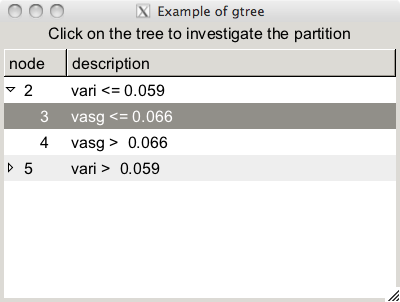
\includegraphics[width=.5\textwidth]{ex-gWidgets-gtree}
  \caption{GUI to explore return value of a model fit by the \code{party}  package.}
  \label{fig:ex-gWidgets-gtree-party}
\end{figure}


We make a simple GUI to show the widget (Figure~\ref{fig:ex-gWidgets-gtree-party})
\begin{Schunk}
\begin{Sinput}
 w <- gwindow("Example of gtree")
 g <- ggroup(cont=w, horizontal=FALSE)
 l <- glabel("Click on the tree to investigate the partition", 
             cont=g)
 tr <- gtree(offspring, cont=g, expand=TRUE)
\end{Sinput}
\end{Schunk}

A single click is used to expand the tree, here we create a binding to
a double click event to create a basic graphic. The \pkg{party}
vignette shows how to make more complicated -- and meaningful --
graphics for this model fit.
\begin{Schunk}
\begin{Sinput}
 addHandlerDoubleclick(tr, handler=function(h,...) {
   node <- as.numeric(svalue(h$obj))
   if(nodes(gt, node)[[1]]$terminal) {   # if terminal plot
     weights <- as.logical(nodes(gt,node)[[1]]$weights)
     plot(response(gt)[weights, ])
   }})
\end{Sinput}
\end{Schunk}
\end{example}





\section{Actions, menus and toolbars}
\label{sec:gWidgets-acti-menus-toolb}


Actions are non-graphical objects representing an application command
that is executable through one or more widgets. Actions in
\pkg{gWidgets} are created through the \constructor{gaction}
constructor. The arguments are \argument{label}{gaction},
\argument{tooltip}{gaction}, \argument{icon}{gaction},
\argument{key.accel}{gaction},~\footnote{The key accelerator
  implementation varies depending on the underlying toolkit. }
\argument{parent}{gaction} and the standard
\argument{handler}{gaction} and \argument{action}{gaction}. 

The label appears as the text on a button, the menu item or toolbar
text, whereas the icon will decorate the same if possible. For some
toolkits, the tooltip pops up when the mouse hovers. The \code{parent} argument is used to
specify a widget whose toplevel container will process the shortcut.

\paragraph{methods}
The main methods for actions are \method{svalue\ASSIGN}{gaction} to
set the label text and \method{enabled\ASSIGN}{gaction} to adjust
whether the widget is sensitive to user input. All proxies of the
action are set through one call. There is no method to invoke the action.

\paragraph{buttons}
An action can be assigned to a button by setting it as the
\argument{action}{gbutton} argument of the \code{gbutton} constructor,
in which case all other arguments for the constructor are ignored.

\begin{Schunk}
\begin{Sinput}
 w <- gwindow("gaction example")
 a <- gaction("click me", tooltip="Click for a message", 
              icon="ok", 
              handler=function(h, ...) {
                print("Hello")
              },
              parent=w)
 b <- gbutton(action=a, cont=w)
 ## .. to change
 enabled(a) <- FALSE                     # can't click now
\end{Sinput}
\end{Schunk}
%%
Action handlers do not have the sender object (\code{b} above)
passed back to them.

% Instead, one uses the \argument{action}{gaction} argument to
% parameterize the call.



\subsection{Toolbars}
\label{sec:gWidgets-toolbars}
Toolbars and menubars are implemented in \pkg{gWidgets} using
\code{gaction} items. Both are specified using a named
list of action components. 

For a toolbar, this list has a simple structure. Each named component
either describes a toolbar item or a separator, where the toolbar
items are specified by \code{gaction} instances and separators by
\code{gseparator} instances with no container specified.

For example. Here we first define some actions:
\begin{Schunk}
\begin{Sinput}
 stub <- function(h,...) gmessage("called handler", parent=w)
 actlist = list(
   new = gaction(label="new", icon="new", 
     handler = stub, parent = w),
   open = gaction(label="open", icon="open", 
     handler = stub, parent = w),
   save = gaction(label="save", icon="save", 
     handler = stub, parent = w),
   save.as = gaction(label="save as...", icon="save as...", 
     handler = stub, parent = w),
   quit = gaction(label="quit", icon="quit", 
     handler = function(...) dispose(w), parent = w),
   cut = gaction(label="cut", icon="cut", 
     handler = stub, parent = w)
   )
 
\end{Sinput}
\end{Schunk}

Then a toolbar list might look like:
\begin{Schunk}
\begin{Sinput}
 w <- gwindow("gtoolbar example")
 tl <- c(actlist[c("new","save")], 
         sep=gseparator(), 
         actlist["quit"])
 tb <- gtoolbar(tl, cont=w)
 gtext("Lorem ipsum ...", cont=w)
\end{Sinput}
\end{Schunk}


The \constructor{gtoolbar} constructor takes the list as its first
argument.  As toolbars belong to the window, the corresponding
\pkg{gWidgets} objects use a \constructor{gwindow} object as the
parent container. (Some of the toolkits relax this to allow other containers.)  The argument
\argument{style}{gtoolbar} can be one of \qcode{both}, \qcode{icons},
\qcode{text}, or \qcode{both-horiz} to specify how the toolbar is
rendered. 


\subsection{Menubars, popup menus}
\label{sec:gWidgets-menubars}

Menubars and popup menus are specified in a similar manner as toolbars with menu items
being defined through \code{gaction} instances, and visual separators
by \code{gseparator} instances. Menus differ from toolbars, as
submenus require a nested structure. This  is specified using a
nested list as the component to describe the sub menu. The lists all
have named components. In this case, the corresponding name is used to
label the submenu item. For menu bars, it is typical that all the
top-level components be lists, but for popup menus, this wouldn't
necessarily be the case.

A example of such a list might be
\begin{Schunk}
\begin{Sinput}
 ml <- list(file = list(
              new = actlist$new,
              open = actlist$open,
              save = actlist$save,
              "save as..." = actlist$save.as,
              sep=gseparator(),
              quit = actlist$quit
              ),
            edit = list(
              cut = actlist$cut
              )
            )
 
\end{Sinput}
\end{Schunk}


Figure~\ref{fig:fig-gWidgets-menubar-disabled} shows this simple GUI
using \pkg{gWidgetsRGtk2}.  Under Mac OS X, with a native toolkit,
menubars may be drawn along the top of the screen, as is the custom of
that OS.

\begin{figure}
  \centering
  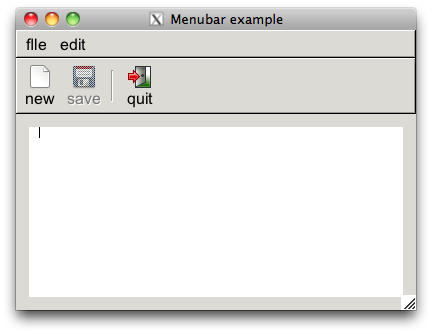
\includegraphics[width=.5\textwidth]{fig-gWidgets-menubar-disabled.png}
  \caption{Menubar and toolbar decorating a basic text editing
    widget. The ``Save'' icon is disabled, as there is no text typed
    in the buffer.}
  \label{fig:fig-gWidgets-menubar-disabled}
\end{figure}

\paragraph{Menubar and Toolbar Methods}
The main methods for toolbar and menubar instances are
the \method{svalue}{gmenu} method which will return the list. Whereas, the
\method{svalue\ASSIGN}{gmenu} method can be used to redefine the
menubar or toolbar. Use the \method{add}{gmenu} method to append to an
existing menubar or toolbar, again using a list to specify the new items.


Here we show how to disable groups of actions. Suppose, we want to
disable the saving and cut actions if there are no characters in the
text buffer, then we could use this handler:

\begin{Schunk}
\begin{Sinput}
 noChanges <- c("save","save.as","cut")
 keyhandler <- function(...) {
   for(i in noChanges)
     enabled(actlist[[i]]) <- (nchar(svalue(txt)) > 0)
 }
 addHandlerKeystroke(txt, handler=keyhandler)
 keyhandler()
\end{Sinput}
\end{Schunk}

% \begin{example}{Menubar and toolbar example}{ex-gWidgets-menu-tool-status-bars}
%   \SweaveInput{ex-gWidgets-menu-tool-status-bars}
% \end{example}

\paragraph{Popup menus}

Popup menus can be created for a right click event through the
\constructor{add3rdMousePopupmenu} constructor. (Or
\kbd{control-button-1} for Mac OS X.) This constructor has arguments
\code{obj} to specify a widget, like a button, to initiate the popup,
\argument{menulist}{gmenu} to specify the menu and optionally an
\argument{action}{gmenu} argument.


\begin{example}{Popup menus}{ex-gWidgets-context-menus}
  This example shows how to add a simple popup menu to a button.
\begin{Schunk}
\begin{Sinput}
 w <- gwindow("Popup example")
 b <- gbutton("click me or right click me", cont=w, 
              handler=function(h, ...) {
                cat("You clicked me\n")
              })
 f <- function(h,...) cat("you right clicked on", h$action)
 mbList <- list(one = gaction("one", action="one", handler=f),
                two = gaction("two", action="two", handler=f)
                )
 add3rdMousePopupmenu(b, mbList)
\end{Sinput}
\end{Schunk}

\end{example}












\chapter{\pkg{gWidgets}: R-specific  widgets}
\label{cha:compound-widgets}
The \pkg{gWidgets} package provides some \R\/ specific widgets for
producing GUIs. Table~\ref{tab:gWidgets-compound-widgets} lists them.


\begin{table}
\centering
\label{tab:gWidgets-compound-widgets}
\caption{Table of constructors for \R-specific widgets in \pkg{gWidgets}}
\begin{tabular}{@{}lp{0.7\textwidth}@{}}
\toprule

Constructor&Description\\
\midrule
\constructor{ggraphics}&Embeddable graphics device\\\constructor{ggraphicsnotebook}&Notebook for multiple devices\\\constructor{gdf}&Data frame editor\\\constructor{gdfnotebook}&Notebook for multiple \code{gdf} instances\\\constructor{gvarbrowser}&GUI for browsing variables in the workspace\\\constructor{gcommandline}&Command line widget\\\constructor{gformlayout}&Creates a GUI from a list specifying layout\\\constructor{ggenericwidget}&Creates a GUI for a function based on its formal arguments or a defining list
\\ \bottomrule
\end{tabular}
\end{table}
% \begin{table}
%   \centering
%   \begin{tabular}{l@{\quad}p{.75\textwidth}}
% %    \toprule
%     \constructor{gcommandline} & Command line widget\\ 
%     \constructor{gvarbrowser} & GUI for browsing variables in the workspace\\
% %    \constructor{gdfnotebook} & A notebook of data frames\\
% %    \constructor{ggraphicsnotebook} & A notebook for graphics objects\\
%     \constructor{ghelp} & GUI for a help page\\
%     \constructor{ghelpbrowser} & A help browser\\
%     \constructor{gformlayout} & Uses list to specify layout of a GUI\\
%     \constructor{ggenericwidget} & Creates a GUI for a function based
%     on its formal arguments or a defining list\\
%     \bottomrule
%   \end{tabular}
%   \caption{Table of compound widgets provided by \pkg{gWidgets}}
%   \label{tab:gWidgets-compound-widgets}
% \end{table}


\section{A graphics device}
\label{sec:gWidgets-graphics-device}

Some toolkits support an embeddable graphics device (\pkg{gWidgetsRGtk2}
through \pkg{cairoDevice}, \pkg{gWidgetsQt} through \pkg{qtutils}). In which case, the \constructor{ggraphics}
constructor produces a widget that can be added to a container. The
arguments \argument{width}{ggraphics}, \argument{height}{ggraphics},
\argument{dpi}{ggraphics}, and \argument{ps}{ggraphics} are similar to
other graphics devices.

%% current device
When working with multiple devices, it becomes necessary to switch
between devices. A mouse click in a \code{ggraphics} instance will
make that device the current one. Otherwise, the
\method{visible\ASSIGN}{ggraphics} method can be used to set the
object as the current device.  The \constructor{ggraphicsnotebook}
creates a notebook that allows the user to easily navigate multiple
graphics devices.




%% handlers
The default handler for the widget is set by
\method{addHandlerClicked}{ggraphics}. The coordinates of the mouse
click, in user coordinates, are passed to the handler in the
components \code{x} and \code{y}. As well, the method
\method{addHandlerChanged}{ggraphics} is used to assign a handler to
call when a region is selected by dragging the mouse. The components
\code{x} and \code{y} describe the rectangle that was traced out,
again in user coordinates.
\\

This shows how the two can be used:
\begin{Schunk}
\begin{Sinput}
 library(gWidgets); options(guiToolkit="RGtk2")
 w <- gwindow("ggraphics example", visible=FALSE)
 g <- ggraphics(cont=w)
 x <- mtcars$wt; y <- mtcars$mpg
 #
 addHandlerClicked(g, handler=function(h, ...) {
   cat(sprintf("You clicked %.2f x %.2f\n", h$x, h$y))
 })
 addHandlerChanged(g, handler=function(h,...) {
   rx <- h$x; ry <- h$y
   if(diff(rx) > diff(range(x))/100 && 
      diff(ry) > diff(range(y))/100) {
     ind <- rx[1] <= x & x <= rx[2] & ry[1] <=y & y <= ry[2]
     if(any(ind))
       print(cbind(x=x[ind], y=y[ind]))
   }
 })
 visible(w) <- TRUE
 #
 plot(x, y)
\end{Sinput}
\end{Schunk}
%

The underlying toolkits may pass in more information about the event,
such as whether a modifier key was being pressed, but this isn't
toolkit independent.

\paragraph{Using tkrplot} The \pkg{tkrplot} provides a means to embed
graphics in \code{Tk} GUIs, but is not a graphics device. As such,
there is no \code{ggraphics} implementation in
\pkg{gWidgetstcltk}. You can embed \code{tkrplot} though. The
following is a simple modification of the example from the help page for \code{tkrplot}:

\begin{Schunk}
\begin{Sinput}
 options(guiToolkit="tcltk"); require(tkrplot)
 w <- gwindow("How to embed tkrplot", visible=FALSE)
 g <- ggroup(cont=w, horizontal=FALSE)
 bb<-1
 img <-tkrplot(getToolkitWidget(g), 
               fun=function() plot(1:20,(1:20)^bb))
 add(g, img)
\end{Sinput}
\begin{Soutput}
<Tcl>  
\end{Soutput}
\begin{Sinput}
 f<-function(...) {
   b <- svalue(sl)
   print(b)
   if (b != bb) {
     bb <<- b
     tkrreplot(img)
   }
 }
 sl <- gslider(from=0.05, to=2, by=0.05, cont=g, 
               handler=f, expand=TRUE)
 visible(w) <- TRUE
 
\end{Sinput}
\end{Schunk}


%% XXXX Move this example somewhere COMPONENT PROGRAMMING
\begin{example}{A GUI for filtering and visualizing a data set}{ex:gWidgets-spotfire}
%% Example of a spotfire like interface

\begin{figure}
  \centering
  \includegraphics[width=.6\textwidth]{fig-gWidgets-spotfire-gui}
  \caption{A GUI to filter a data frame and display an accompanying graphic.}
  \label{fig:gWidgets-spotfire-gui}
\end{figure}
A common GUI application for data analysis consists of means to
visualize, query, aggregate and filter a data set. This example shows
how one can create such a GUI using \pkg{gWidgets} featuring an
embedded graphics device. In addition a visual display of the filtered
data, and a means to filter, or narrow, the data that is under
consideration, is presented (Figure~\ref{fig:gWidgets-spotfire-gui}).
Although, our example is not too feature rich, it illustrates a
framework that can easily be extended.


This example is centered around filtering a data set, we choose a
convenient one and give it a non-specific name.
\begin{Schunk}
\begin{Sinput}
 data("Cars93", package="MASS")
 x <- Cars93
\end{Sinput}
\end{Schunk}

We use a notebook to hold two tabs, one to give information and one
for the main GUI. This basic design comes from the spotfire demos at \url{tibco.com}.
\begin{Schunk}
\begin{Sinput}
 w <- gwindow("Spotfire example", visible=FALSE)
 nb <- gnotebook(cont=w)
\end{Sinput}
\end{Schunk}


We use a simple label for information, although a more detailed
description would be warranted in an actual application.

\begin{Schunk}
\begin{Sinput}
 descr <- glabel(gettext("A basic GUI to explore a data set"), 
                 cont=nb, label=gettext("About"))
\end{Sinput}
\end{Schunk}
%
Now we specify the layout for the second tab. This is a nested layout
made up of three box containers. The first, \code{g}, uses a
horizontal layout in which we pack in box containers that will use a
vertical layout.

\begin{Schunk}
\begin{Sinput}
 g <- ggroup(cont=nb, label=gettext("Explore..."))
 lg <- ggroup(cont=g, horizontal=FALSE) 
 rg <- ggroup(cont=g, horizontal=FALSE)
\end{Sinput}
\end{Schunk}

The left side will contain an embedded graphic device and a view of
the filtered data. The \constructor{ggraphics} widget provides the
graphic device.
\begin{Schunk}
\begin{Sinput}
 ggraphics(cont = lg)
\end{Sinput}
\end{Schunk}

Our view of the data is provided by the \constructor{gtable} widget,
which facilitates the display of a data frame. The last two arguments
allow for multiple selection (for marking points on the graphic) and
for filtering through the \method{visible\ASSIGN}{gtable} method.
In addition to the table, we add a label to display the number of
cases being shown. This label is packed into a box container, and
forced to the right side through the \method{addSpring}{ggroup} method
of the box container.
\begin{Schunk}
\begin{Sinput}
 tbl <- gtable(x, cont = lg, multiple=TRUE, filter.FUN="manual")
 size(tbl) <- c(500, 200)                # set size
 labelg <- ggroup(cont = lg)
 addSpring(labelg)
 noCases <- glabel("", cont = labelg)
\end{Sinput}
\end{Schunk}

The right panel is used to provide the user a means to filter the
display. We place the widgets used to do this within a frame to guide
the user.
\begin{Schunk}
\begin{Sinput}
 filterg <- gframe(gettext("Filter by:"), cont = rg, expand=TRUE)
\end{Sinput}
\end{Schunk}
The controls are layed out in a grid. We have two here to filter by:
type and the number of cylinders.
\begin{Schunk}
\begin{Sinput}
 lyt <- glayout(cont=filterg)
 l <- list() # store widgets
 lyt[1,1] <- "Type:"
 lyt[1,2] <- (l$Type <- gcombobox(c("", levels(x$Type)), 
                                  cont=lyt))
 lyt[2,1] <- "Cylinders:"
 lyt[2,2] <- (l$Cylinders <- 
              gcombobox(c("", levels(x$Cylinders)), cont=lyt))
\end{Sinput}
\end{Schunk}
%
Of course, we could use many more criteria to filter by. The above
filters are naturally represented by a combo box. However, one could
have used many different styles, depending on the type of data. For
instance, one could employ a checkbox to filter through Boolean data,
a checkbox group to allow multiple selection, a slider to pick out
numeric data, or a text box to specify filtering by a string. The type
of data dictates this. In this example it isn't needed, but since the
layout is done, we might have code to initialize the controls in the
filter. Adding such a call, makes it easy to save the state of the GUI.

%% handlers
We now move on to the task of making the three main components -- the
display, the table and the filters -- interact with each other. We
keep this example simple, but note that if we were to extend the
example we would likely write using the observer pattern introduced in
Example~\ref{ex-gWidgets-ws-browser} as that makes it easy to decouple
the components of an interface. As it is we define function calls to
a) update the data frame when the filters change and b) update the
graphic.

For the first, we need to compute a logical variable indicating which
rows are to be displayed.  Within the definition of the following function, we
use the global variables \code{l}, \code{tbl} and \code{noCases}.
\begin{Schunk}
\begin{Sinput}
 updateDataFrame <- function(...) {
   vals <- lapply(l, svalue)
   vals <- vals[vals != ""] 
   out <- sapply(names(vals), function(i) x[[i]] == vals[[i]])
   ind <- apply(out, 1, function(x) Filter("&&", x))
   ## update table
   visible(tbl) <- ind
   ## update label
   nsprintf <- function(n, msg1, msg2,...)
     ngettext(n, sprintf(msg1, n), sprintf(msg2,n), ...)
   svalue(noCases) <- nsprintf(sum(ind), "%s case", "%s cases")
 }
\end{Sinput}
\end{Schunk}

% %% methods
% The \method{visible\ASSIGN}{gtable} and \method{svalue\ASSIGN}{glabel}
% methods change the underlying widgets. The generic
% \meth{svalue\ASSIGN} is used to change the primary value for a widget
% (and \meth{svalue} returns this value). In the above, we see these
% methods used to get the values from the combo boxes and to set the text
% in the label. The \meth{visible\ASSIGN} method is another generic. In
% this example it is used to specify which rows of the data are actually
% displayed by the widget.

This next function is used to update the graphic. A real application
would provide a more compelling plot.
\begin{Schunk}
\begin{Sinput}
 updateGraphic <- function(...) {
   ind <- visible(tbl)
   if(any(ind))
     plot(MPG.city ~ Weight, data=x[ind,])
   else
     plot.new()
 }
\end{Sinput}
\end{Schunk}

We now add a handler to be called whenever one of our combo boxes is
changed. This handler simply calls both our update functions.
\begin{Schunk}
\begin{Sinput}
 f <- function(h, ...) {
   updateDataFrame()
   updateGraphic()
 }
 sapply(l, addHandlerChanged, handler=f)
\end{Sinput}
\end{Schunk}
%
For the data display, we wish to allow the user to view individual cases
by clicking on a row of the table. The following will do so.

\begin{Schunk}
\begin{Sinput}
 addHandlerClicked(tbl, handler=function(h,...) {
   updateGraphic()
   ind <- svalue(h$obj, index=TRUE)
   points(MPG.city ~ Weight, cex=2, col="red", pch=16, 
          data=x[ind,])
 })
\end{Sinput}
\end{Schunk}
%
We could also use the \method{addHandlerChanged}{ggraphics} method to
add a handler to call when the user drags our a region in the graphics
device, but leave this for the interested reader.


Finally, we draw the GUI with an initial graphic
\begin{Schunk}
\begin{Sinput}
 visible(w) <- TRUE
 updateGraphic()
\end{Sinput}
\end{Schunk}
\end{example}

%%% 
% \begin{example}{A GUI to explore a data set}{ex-gWidgets-baseball}
%   \SweaveInput{ex-gWidgets-baseball-RGtk2.Rnw}
% \end{example}


\section{A data frame editor}
\label{sec:gWidgets-an-editor-tabular}

The \constructor{gdf} constructor returns a widget for editing data
frames. The intent is for each toolkit to produce a widget at least as
powerful as the \function{data.entry} function. The implementations
differ between toolkits, with some offering much more. We describe
what is in common below.~\footnote{ For \pkg{gWidgetstcltk}, there is
  no native widget for editing tabular data, so the \code{tktable}
  add-on widget is used (\url{tktable.sourceforge.net}). A warning
  will be issued if this is not installed. Again, as with
  \function{gtable}, the widget under \pkg{gWidgetstcltk} is slower,
  but can load a moderately sized data frame in a reasonable time. 
  
  For \pkg{gWidgetsRGtk2} there is also the \constructor{gdfedit}
  widget which can handle very large data sets and has many improved
  usability features. The \pkg{gWidgets} function merely wraps the
  \function{gtkDfEdit} function from \pkg{RGtk2Extras}. This function
  is not exported by \pkg{gWidgets}, so the toolkit package must be
  loaded before use. }


The constructor has its main argument \argument{items}{gdf} to specify the data
frame to edit. A basic usage might be:

\begin{Schunk}
\begin{Sinput}
 w <- gwindow("gdf example")
 df <- gdf(mtcars, cont=w)
 ## ... make some edits ...
 newDataFrame <- df[,]                   # store changes
\end{Sinput}
\end{Schunk}
%

Some toolkits render columns differently for different data types, and
some toolkits use character values for all the data, so values must be
coerced back when transferring to \R\/ values. As such, column types
are important. Even if one is starting with a $0$-row data frame, the
columns types should be defined as desired. Also, factors and
character types may be treated differently, although they may render
in a similar manner.

\paragraph{Methods} The \method{svalue}{gdf} method will return the
selected values or selected indices if \code{index=TRUE} is given. The
\method{svalue\ASSIGN}{gdf} method is used to specify the selection by
index. This is a vector or row indices, or for some toolkits a list
with components \code{rows} and \code{columns} indicating the
selection to mark.  The \method{[}{gdf} and \method{[\ASSIGN}{gdf}
methods can be used to extract and set values from the data frame by
index. As with \code{gtable}, these are not as flexible as for a data
frame. In particular, it may not be possible to change the type of a
column, or add new rows or columns through these methods. Using no
indices, as in the above example with \code{df[,]}, will return the
current data frame. The current data frame can be completely replaced,
when no indices are specified in the replacement call.

There are also several methods defined that follow those of a data
frame: \method{dimnames}{gdf}, \method{dimnames\ASSIGN}{gdf},
\method{names}{gdf}, \method{names\ASSIGN}{gdf}, and
\method{length}{gdf}.

The following methods can be used to assign handlers:
\method{addHandlerChanged}{gdf} (cell changed),
\method{addHandlerClicked}{gdf},
\method{addHandlerDoubleclick}{gdf}. Some toolkits also have
\method{addHandlerColumnClicked}{gdf},
\method{addHandlerColumnDoubleclick}{gdf}, and
\method{addHandlerColumnRightclick}{gdf} implemented.
\\


The \constructor{gdfnotebook} constructor produces a notebook that can
hold several data frames to edit at once.





\subsection{Workspace browser}
\label{sec:gWidgets-workspace-browser}

A workspace browser is constructed by \code{gvarbrowser}, providing a
means to browse and select the objects in the current global
environment. This workspace browser uses a tree widget to display the
items and their named components.

The \code{svalue} method returns the name of the currently selected value
using \code{\$} to refer to child elements.  One can call
\code{svalue} on this string to get the \R\/ object.

The default \argument{handler}{gvarbrowser} object calls
\code{do.call} on the object for the function specified by name
through the \argument{action}{gvarbrowser} argument. (The default is
to print a \code{summary} of the object.) This handler is called on a
double click. A single click is used for selection. One can pass in
other handler functions if desired.  


The \method{update}{gvarbrowser} method will update the list of items
being displayed.  This can be time consuming. Some heuristics
are employed to do this automatically, if the size of the workspace is
modest enough. Otherwise it can be done by programmatically.

\begin{example}{Using drag and drop with \pkg{gWidgets}}{ex-gWidgets-drag-and-drop}
  We use the drag and drop features to create a means to plot
  variables from the workspace browser.  Our basic layout is fairly
  simple. We place the workspace browser on the left, and on the right
  have a graphic device and few labels to act as drop targets.
\begin{Schunk}
\begin{Sinput}
 w <- gwindow("Drag and drop example")
 g <- ggroup(cont=w)
 vb <- gvarbrowser(cont=g)
 g1 <- ggroup(horizontal=FALSE, cont=g, expand=TRUE)
 ggraphics(cont=g1)
 xlabel <- glabel("", cont=g1)
 ylabel <- glabel("", cont=g1)
 clear <- gbutton("clear", cont=g1)
\end{Sinput}
\end{Schunk}
%
We create a function to initialize the interface.
\begin{Schunk}
\begin{Sinput}
 init_txt <- "<Drop %s variable here>"
 initUI <- function(...) {
   svalue(xlabel) <- sprintf(init_txt, "x")
   svalue(ylabel) <- sprintf(init_txt, "y")
   enabled(ylabel) <- FALSE
 }
 initUI()                                # initial call
\end{Sinput}
\end{Schunk}
%
Separating this out allows us to link it to the clear button.
\begin{Schunk}
\begin{Sinput}
 addHandlerClicked(clear, handler=initUI)
\end{Sinput}
\end{Schunk}
%
Next, we write a function to update the user interface. As we didn't
abstract out the data from the GUI,
we need to figure out which state the GUI is currently in by
consulting the text in each label.
\begin{Schunk}
\begin{Sinput}
 updateUI <- function(...) {
   if(grepl(svalue(xlabel), sprintf(init_txt, "x"))) {
     ## none set
     enabled(ylabel) <- FALSE
   } else if(grepl(svalue(ylabel), sprintf(init_txt, "y"))) {
     ## x, not y
     enabled(ylabel) <- TRUE
     x <- eval(parse(text=svalue(xlabel)), envir=.GlobalEnv)
     plot(x, xlab=svalue(xlabel))
   } else {
     enabled(ylabel) <- TRUE    
     x <- eval(parse(text=svalue(xlabel)), envir=.GlobalEnv)
     y <- eval(parse(text=svalue(ylabel)), envir=.GlobalEnv)
     plot(x, y, xlab=svalue(xlabel), ylab=svalue(ylabel))
   }
 }
\end{Sinput}
\end{Schunk}

Now we add our drag and drop information.  Drag and drop support in
\pkg{gWidgets} is implemented through three methods: one to set a
widget as a drag source (\generic{addDropSource}), one to set a widget
as a drop target (\generic{addDropTarget}), and one to call a handler
when a drop event passes over a widget (\generic{addDropMotion}).
  

The \generic{addDropSource} method needs a widget and a handler to
call when a drag and drop event is initiated. This handler should
return the value that will be passed to the drop target. The default
value is that returned by calling \code{svalue} on the object. In this
example we don't need to set this, as \generic{gvarbrowser} already
calls this with a drop data being the variable name using the dollar
sign notation for child components.
    
The \generic{addDropTarget} method is used to allow a widget to
receive a dropped value and to specify a handler to call when a value
is dropped. The \code{dropdata} component of the first argument of the
callback, \code{h}, holds the drop data. In our example below we use
this to update the receiver object, either the $x$ or $y$ label.

\begin{Schunk}
\begin{Sinput}
 dropHandler <- function(h,...) {
   svalue(h$obj) <- h$dropdata
   updateUI()
 }
 addDropTarget(xlabel, handler=dropHandler)
 addDropTarget(ylabel, handler=dropHandler)
\end{Sinput}
\end{Schunk}


The \generic{addDropMotion} registers a handler for when a drag event
passes over a widget. We don't need this for our GUI.
    
\end{example}



\subsection{Help browser}
\label{sec:gWidgets-help-browser}

The \constructor{ghelp} constructor produces a widget for showing help
pages using a notebook container. Although \R\/ now has excellent
ways to dynamically view help pages through a web browser (in
particular the \pkg{helpr} package and the standard built-in help
page server) this widget provides a light-weight alternative that can
be embedded in a GUI.

To add a help page, the \method{add}{ghelp} method is used,
where the \code{value} argument describes the desired page. This can
be a character string containing the topic, a character string of the
form \code{package:::topic} to specify the package, or a list with
named components \code{package} and \code{topic}.  The
\method{dispose}{ghelp} method of notebooks can be used to remove the
current tab.
\\

The \constructor{ghelpbrowser} constructor produces a stand-alone
GUI for displaying help pages, running examples from the help pages or
opening vignettes provided by the package. This GUI provides its own
top-level window and does not return a value for which methods are defined.



\subsection{Command line widget}
\label{sec:gWidgets-command-line-widget}



A simple command line widget is created by the
\constructor{gcommandline} constructor. This is not meant as a
replacement for any of \R's command lines, but is provided for
light-weight usage. A text box allows users to type in \R\/
commands. The programmer may issue commands to be evaluated and
displayed through the \method{svalue\ASSIGN}{gcommandline} method. The
\code{value} assigned is a character string holding the commands. If
there is a \code{names} attribute, the results will be assigned to a variable
in the global workspace with that name. The \code{svalue} and \code{[}
methods return the command history.

\subsection{Simplifying creation of dialogs}
\label{sec:gWidgets-designing-forms}

The \pkg{gWidgets} package has two means to simplify the creation of
GUIs.~\footnote{The \pkg{traitr} package provides another, but is not
  discussed here. The \pkg{fgui} package can do such a thing for
  \pkg{tcltk}.}  The \code{gformlayout} constructor takes a list
defining a layout and produces a GUI, the \code{ggenericwidget}
constructor can take a function name and produce a GUI based on the
formal arguments of the function. This too uses a list, which can be
modified by the user before the GUI is constructed. We leave the
details to their manual pages.

% \subsubsection{Laying out a form}
% \label{sec:gWidgets-laying-out-form}

% % ML: replaced 'component' with 'element' for components of list, to
% % distinguish them from components of the GUI

% % ML: this is another place where it would be good to see the example first
% %% JV: Good ideas, done.

% The \constructor{gformlayout} constructor takes a list defining a
% layout and creates the specified widgets. The design borrows from the
% \code{extjs} javascript libraries for web programming, where a similar
% function can be used to specify the layout of web forms. Several
% toolkits have a means to specify a layout using XML (eg. \GTK{}
% Builder and \Qt{} Assistant); this implementation uses a list, under
% the assumption that it is more familiar to the \R\/ user. By defining
% the layout ahead of time, pieces of the layout can be recycled for
% other layouts.

% A simple example would be
% <<>>=
% l <- list(type="ggroup",
%           horizontal=TRUE,
%           children=list(
%             list(type="glabel",
%                  text="x:"),
%             list(name="x",
%                  label="asdfas",
%                  type="gedit",
%                  text="initial text"),
%             list(type="glabel",
%                  text="state:"),
%             list(name="y",
%                  type="gcombobox",
%                  items=state.name)
%             )
%           )
% w <- gwindow("glayout example")
% f <- gformlayout(l, cont=w)

% @ 


% To define the layout, each list element is specified using a 
% named. The \code{type} element indicates the component
% to be created, as a string. This can be the name of a container
% constructor, a widget constructor or the special value
% \code{"fieldset"}. Field sets are used to group a set of common
% controls. 

% The list defining each GUI component has named elements to pass to the
% constructor, such as \code{text} and \code{items} in the above
% example, and named elements used by the \generic{gformlayout}
% constructor. For example, 
% the \code{name} element when specified, allows that
% component to be referenced through \method{svalue}{gformlayout},
% which returns the form's values in a list, or \method{[}{gformlayout},
% which returns the components in a list.

% If the type is a container or fieldset, then the \code{children}
% element is a list whose elements specify the children as
% above. Except for fieldsets, these children can contain other
% containers or controls. Fieldsets only allow controls as children.


% %% fields set and labels.
% For \code{fieldset}s the \code{label} element adds a descriptive label
% to the layout. The \code{label.pos} element controls the placement of
% the label. The value \code{"top"} places the label on top of the
% widget, while \code{"side"}, the default, puts it on the side. The
% \code{label.font} element specifies the font properties of the label,
% as with the \meth{font\ASSIGN} method.

% Parts of the form can be made to depend on other parts. For example, 
% whether a component is enabled or not may be controlled by the by \code{depends.on},
% \code{depends.FUN}, and \code{depends.signal} elements. If the
% \code{depends.on} element specifies the name of a previous component,
% then the function \code{depends.FUN} will be consulted when the signal
% specified by \code{depends.signal} is emitted. This uses the
% \code{addHandlerXXX} names with a default value of
% \code{addHandlerChanged}. The \code{depends.FUN} function should take a single
% argument consisting of the value returned by \code{svalue} when called
% on the widget specified through \code{depends.on}. This function
% should return a logical indicating if the widget is enabled or not.

% The constructor returns an object with just a few methods. In addition to
% \meth{svalue} and \meth{[}, the \method{names}{gformlayout} method
% returns the names of the widgets in the list.

% %% JV: this example will be in the package, but perhaps not needed here.
% % \begin{example}{The \code{gformlayout} constructor}{ex-gWidgets-gformlayou}
% %   \SweaveInput{ex-gWidgets-formlayout}
% % \end{example}

% \subsubsection{Creating a GUI for a function}
% \label{sec:gWidgets-autom-creat-gui}

% The \constructor{ggenericwidget} constructor creates a GUI for
% invoking a given function. The GUI is derived from the formal
% arguments. The \pkg{fgui} package provides a similar function, with
% some more features, although limited to the \pkg{tcltk} toolkit.


% The usage is straightforward. To make a GUI for a function is as
% simple as:
% <<>>=
% f <- function(x=1, variable="a") {
%   print("Something with x and variable")
% }
% g <- ggenericwidget(f, cont=gwindow())
% @ 
% %
% The formal arguments of an S3 method may be different from those of
% its generic. For instance, those for the \code{t.test} generic are
% much different (and less useful for this purpose) than the
% \code{t.test.default} method for numeric values for \code{x}. Knowing
% this, a useful GUI can be quickly created for the \code{t.test} with
% the commands:
% <<>>=
% w <- gwindow("t.test through ggenericwidget")
% f <- stats:::t.test.default; 
% widget <- ggenericwidget("f", cont=w)
% @ 


% The implementation has two stages. The first creates a list
% specifying the layout of the GUI and the second actually constructs
% the GUI. This list is different from that used by \code{gformlayout}. It
% does not provide as much flexibility and is described in the help page
% for \code{ggenericwidget}. This list can dumped to a text file, edited if desired and then
% sourced in later. For example:

% <<results=hide>>=
% tmp <- tempfile()
% cat(gWidgets:::autogenerategeneric(f), file=tmp)
% ## ... do some edits ...
% source(tmp)
% w <- gwindow("Another ggeneric widget example")
% ggenericwidget(f.LIST, cont=w)          # made by autogenerategeneric
% @ 



\XXX{Need to have an example with drag and drop}


%\section{End of chapter notes}
%\label{sec:gWidgets:eoc}





